\documentclass[a4paper, 11pt, normalem]{report}

\usepackage{../../../LaTeX-Templates/Notes}
\usepackage{subfiles}
\usepackage{tensor}
\usetikzlibrary{arrows.meta}
\usetikzlibrary{decorations.markings}
\usetikzlibrary{decorations.pathmorphing}
\tikzset{snake it/.style={decorate,decoration=snake}}

\newcommand\xo{\hat{X}_1}
\newcommand\xt{\hat{X}_2}
\newcommand\hsig{\hat{\sigma}}
\newcommand\hd{\hat{\unl{d}}}
\newcommand\hrho{\hat{\rho}}

%\title{General Relativity \vspace{-20pt}}
%\author{Richard Bower}
%\date{\vspace{-15pt}Epiphany Term 2020}
\rhead{\hyperlink{page.1}{Contents}}

\begin{document}
\begin{titlepage}
    \newcommand{\HRule}{\rule{\linewidth}{0.5mm}}
    \center
    {
\includegraphics[scale=0.5]{../../logo0.png}\hfill{\Large\bfseries Epiphany 2020}}\\[2.5cm]
    \HRule \\[0.7cm]
    {\huge\bfseries General Relativity}\\[0.4cm]
    \HRule \\[1.5cm]

    \begin{minipage}{0.4\textwidth}
        \begin{flushleft} \large
            \emph{Author:} \\ Matthew Rossetter
        \end{flushleft}
    \end{minipage}~
    \begin{minipage}{0.4\textwidth}
        \begin{flushright} \large
            \emph{Lecturer:} \\ Prof. Richard Bower
        \end{flushright}
    \end{minipage}\\[2cm]
    \vfill
    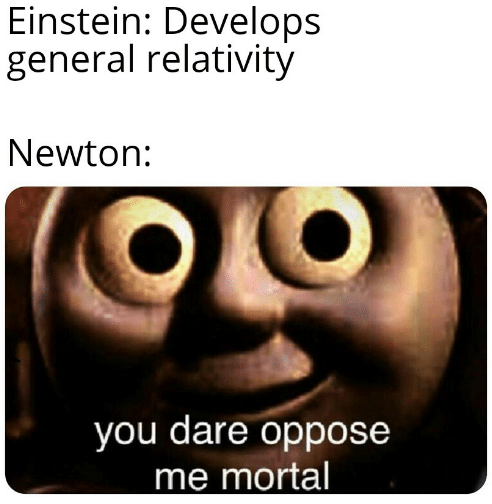
\includegraphics[width=0.7\textwidth]{newt.png}\\[1cm]
    \vfill
\end{titlepage}
\tableofcontents

\chapter{Introduction to GR: The Easy Way}
\section{Special Relativity}
Observers see space and time differently, but the \emph{spacetime interval} is the same for all observers. 
It is a \emph{conserved quantity} and in 3D+time, it is
\begin{align}
    ds^2 &= c^2dt^2 - dx^2 - dy^2 - dz^2.
\end{align}
However, special relativity only works in an inertial frame - it doesn't handle acceleration. 
You will need to revise special relativity and be comfortable using it. 

\section{The Principle of Equivalence}
What is the difference between an accelerated frame without a gravitational field and a stationary frame within a gravitational field? \textbf{Nothing!}
This explains why inertial and gravitational masses are the same. 
\begin{itemize}
    \item \textbf{Inertial mass, $m_i$,} gives the constant of proportionality between force and acceleration, 
        \begin{align}
            F=m_ia.
        \end{align}
    \item \textbf{Gravitational mass, $m_g$,} determines how the object is affected by the force of gravity, 
        \begin{align}
            F \frac{GMm_g}{r^2} = m_gg.
        \end{align}
\end{itemize}
So when an object falls under a gravitational field, we have $a = \frac{m_g}{m_i}g$ and the only way for objects to fall the same way in a gravitational field is if $\frac{m_g}{m_i}=$const.
In electromagnetism, a particle with charge $q$ and inertial mass $m_i$ in a field $\mathcal{E}$ experiences a force $F=q\mathcal{E}$, and acceleration $m_ia$, so $a=\frac{q}{m_i}\mathcal{E}$ and different particles have different values of $\frac{m_g}{m_i}$.
Gravity needs to be the same as being accelerated, i.e. the \textbf{Principle of Equivalence.}
This means \textbf{Acceleration = Gravity} and we should no longer consider gravity a force.

\section{Acceleration}
Circular motion is a nice way to get an accelerated frame since the speed is constant. 
Consider a roundabout:
\begin{itemize}
    \item If stationary, a person measuring the circumference and radius with a ruler gets a ratio of $\frac{c}{r}=2\pi$.
    \item If spinning, if the rule is small enough then it lies along the direction of motion, its length is then shortened and more rules are needed to get round the circumference. Along the radius, the ruler is unaffected as it is perpendicular to the motion, so now $\frac{c}{r}>2\pi$.
\end{itemize}
This is not possible in flat space, but it can be in curved space. 
\begin{itemize}
    \item Zero curvature $\implies C=2\pi r$.
    \item Positive curvature (surface falls away from us) $\implies C<2\pi r$.
    \item Negative curvature (curves away in one direction and together in the other) $\implies C>2\pi r$. In this curvature, the angles of a triangle sum to $<180^\circ$.
\end{itemize}
We must use curved space for accelerating frames!

\section{Curved Space}
On a flat surface, we get a straight line path but on a \emph{curved surface}, we trace out a curved path when we walk in a straight line from our perspective - we may move closer together as if there was an attractive force. 
\textbf{Gravity = acceleration $\implies$ gravity = curvature} - there is no force. 
The `walking normally' paths are constant velocity frames, i.e. inertial frames but in geometric language they are \emph{geodesic paths} - shortest distance between two paths. 
Natural paths (no forces = inertial frame) are `straight lines', geodesics of a curved surface.
Locally, \emph{geodesics} appear straight but over more extended regions of spacetime then geodesics originally receding from each other begin to approach at a rate governed by the curvature of spacetime. 
Warping of spacetime comes from matter/energy: \textbf{Space tells matter how to move, matter tells space how to curve.}
In summary, \textbf{Gravity = Acceleration (EP); Acceleration = Curvature (SR); Gravity = Curvature (GR).}

\section{Implications for Matter}
Mass curves spacetime so energy curves spacetime as $E=mc^2$.
Mass and energy are equivalent - any form of energy adds to the curvature of spacetime which is gravity.
Kinetic energy adds to the response of the particle to gravity, i.e. adds to its mass, so when kinetic energy is a substantial fraction of the rest mass, then additional acceleration will increase the response to gravity of the particles, i.e. increase its mass, which stops the velocity increasing above $c$.

\section{Implications on Light}
Curved space affects everything, even \emph{massless particles} such as light. 
This is not obvious in \emph{Newtonian gravity} as here gravity affects things with mass through
\begin{align}
    F = \frac{GMm}{r^2},\text{ but } a = \frac{F}{m}=\frac{GM}{r^2},
\end{align}
so we could argue that in Newtonian gravity, light has no mass so it is not affected, or that gravitational acceleration is independent of mass so it affects everything. 
Light speed is constant so we would think it is unaffected by gravity. 
In general relativity, light is clearly affected as it travels across curved spacetime so its path will be curved. 
This was seen in first experimental tests of general relativity with light from distant stars which has a project line of sight which lies close to the sun. 
These paths are curved - there are different apparent positions 6 months later when the star is over the other side from the sun (Eddington \emph{solar eclipse}).
The measured deviation of this agrees with general relativity!

We can use this deflected light to determine the mass of a galaxy - this can be direct evidence for \textbf{Dark Matter.}
If we understand the distortion, we can \emph{reconstruct the galaxy} behind a lens and investigate it. 
The object will also be much brighter than without the lens. 

\section{Implications for Matter and Light}
We need gravity to affect light, otherwise we could produce an infinite energy machine - \emph{Pounds-Rebka -Synder experiment.}
Particle dropped from $h$ has energy of rest mass plus $mgh$ at the bottom and converting this to a photon and sending it back up the tower.
If gravity doesn't affect light, it arrives at the top with $h\nu=m_0c^2+m_0gh$, then converting all energy to mass, we get a particle of mass $m_1c^2 = m_0c^2+m_0gh,m_1>m_0$.
We could do this an infinite amount of times and yield infinite energy!
If gravity can affect light, however, then the photon loses the same amount of energy on the way up as the particle gains on the way down - this is \emph{gravitational redshift} which is measurable and general relativity correctly predicts this. 

\section{Gravity Waves}
Space takes a finite time to respond to changes in the distribution of mass and energy. 
In general relativity, gravity does not instantaneously affect everything around it. 
If we have an oscillating distribution of mass, this leads to something like an electromagnetic wave travelling out from the source - a ripple in the structure of spacetime. 
Spacetime is rather stuff, and you need a huge mass to generate a significant deflection. 
We have now detected these waves thanks to LIGO!

\section{Implications: Black Holes}
What happens if gravity is really strong? 
So strong that even a photon can't escape?
We have an \textbf{event horizon} at which point nothing can escape and a singularity is at the centre of this. 

\section{The Way Ahead}
\begin{enumerate}
    \item Understand how to describe curvature, using tensors and \emph{metrics.}
    \item Figure out how mass/energy curves spacetime, using \emph{Einstein's equations.}
    \item How to describe `straight line' \emph{geodesic paths}, using \emph{Lagrangian mechanics.}
\end{enumerate}

\section{Mathematical Toolkit}
We will need complicated maths for this. 
Also a way to characterise the curvature, or shape, of a surface - this will in the \emph{metric.}
The distance between points tells us the shape of the surface, e.g. the \emph{metric for special relativity:}
\begin{align}
    ds^2 &= c^2dt^2-dx^2-dy^2-dz^2 = \begin{pmatrix} c\,dt & dx & dy & dz \end{pmatrix}\begin{pmatrix} 1 & 0 & 0 & 0 \\ 0 & -1 & 0 & 0 \\ 0 & 0 & -1 & 0 \\ 0 & 0 & 0 & -1 \end{pmatrix}\begin{pmatrix} c\,dt \\ dx \\ dy \\ dz\end{pmatrix},
\end{align}
or this can be written as a direct sum:
\begin{align}
    ds^2 &= \sum_{\alpha=0}^3 \sum_{\beta=0}^3 dx(\alpha)\eta(\alpha,\beta)dx(\beta),
\end{align}
where $dx(0)=c\,dt,\; dx(1)=dx,\; dx(2)=dy,\; dx(3)=dz$, and $\eta(\alpha,\beta)=\text{diag}(1,-1,-1,-1)$.
We also use the \textbf{Einstein summation convention}: wherever an expression contains one index as a superscript and the same index as a subscript, then the summation is implied. 
So for the above, we just write
\begin{align}
    ds^2 &= \eta_{\alpha\beta}dx^\alpha dx^\beta.
\end{align}
Simpler but also $\eta_{\alpha\beta}$ contains a lot of new mathematics. 
Next is Tensors, a way of describing physical quantities independent of the coordinate system used to locate them in spacetime.


\chapter{Introduction to Tensors}
\begin{itemize}
    \item Notation
    \item Coordinate transforms
    \item Contravariant tensors
    \item Covariant tensors
\end{itemize}
We need \textbf{tensors} and compact notation to do physics in curved spacetime.

\section{Notation}

Consider the standard vectors in \emph{Cartesian coordinates} and the definition for $\vr$:
\begin{align}
    \vr = x\vec{i} + y\vec{j} + z\vec{k}.
\end{align}
We have the basis vector $\{\vec{i},\vec{j},\vec{k}\}$ and coordinate values $\{x,y,z\}$.
Instead, we can write axes as labelled by indices, i.e. $\{x,y,z\}=\{x^1,x^2,x^3\}$.
Note: $x^2 \neq x*x$.
The 2 is an index, not a power.
If we want to square something, we will write $(x^1)^2 = x^1x^1$.
The \emph{basis vectors} are now $\ve_1,\ve_2,\ve_3$.
We use the shorthand notation that $\{x^i\}$ means all of the set $\{x^1,x^2,x^3\}$.
We can then simplify this further using the \textbf{Einstein summation convention}: wherever an expression contains one index as a superscript and the same index as a subscript, then the summation is implied, so
\begin{align}
    \vr = x^1\ve_1+x^2\ve_2+x^3\ve_3 = \sum_{i=1}^3 x^i\ve_i = x^i\ve_i.
\end{align}
Different letters will imply different things:
\begin{itemize}
    \item Roman letters $i,j,\dots$ - summing over 3D space
    \item Roman letters $a,b,c,\dots$ - summing over ND space
    \item Roman letters $A,B,\dots$ - summing over 2D space
    \item Greek letters $\alpha,\beta,\mu,\nu,\dots$ - summing over 4D spacetime $\{x^0,x^1,x^2,x^3\}$, starting from 0 as time is different slightly, so $\{ct,x^i\}$
\end{itemize}

\section{Coordinate Transformation}
We might want to do various coordinate transformations. 
Up till now, we have often see this denoted as the primed coordinate frame, using \textbf{Lorentz transformations} such as
\begin{align}
    x' = \gamma\left(x-\frac{vct}{c}\right),
\end{align}
where the extra $c$ factor to make time space-like.
Since the prime is similar to a 1, we now use a \emph{bar on the index} to denote a \emph{transformation to a different frame}, so we have
\begin{align}
    x^{\bar{1}} = \gamma\left(x^1-\frac{vx^0}{c}\right),
\end{align}
where the 'bar' indicates new coordinate system.\\
Now thinking about more general spaces with arbitrary curvature. 
Define a point P in some space, and another point a little further called Q; these points have nothing to do with the coordinate system, they exist irrespective of labels. 
Assume they are defined on coordinates $x^a$ with basis vectors $\ve_a$:
\begin{align}
    \vr(P) &= x^a(P)\ve_a, & \vr(Q) &= x^a(Q)\ve_a, 
\end{align}
and the displacement vector which points from P to Q is
\begin{align}
    d\vr &= \left[x^a(Q)-x^a(P)\right]\ve_a = dx^a\ve_a.
\end{align}
Tensor representations in different coordinate systems depend only on the relative orientations and scales on the coordinate axes at that point and not the absolute values of coordinates - $d\vr$ will be the same in all coordinate systems, though its components will be different depending on our choice of coordinates. 
An arbitrary position vector
\begin{align}
    \vr = x^1\ve_1+x^2\ve_2+\dots = x^a\ve_a
\end{align}
has components $x^a$ along whatever basis vectors $\ve_a = \frac{\p\vr}{\p x^a}$ we are using.
We could use this definition to work our what a basis vector is. 
Note: they don't have to be orthogonal or unit vectors - or constant, they could be functions of time.
Transforming to a different coordinate system $x^{\bar{b}}$, the vector is the same vector so
\begin{align}
    \vr=x^a\ve_a=x^{\bar{b}}\ve_{\bar{b}}.
\end{align}
We again get basis vectors from partial derivatives, $\ve_{\bar{b}}=\frac{\p\vr}{\p x^{\bar{b}}}$, and we can transform between these, writing the \emph{new coordinates} as a function of the \emph{old ones}:
\begin{align}
    x^{\bar{1}}=x^{\bar{1}}(x^1,x^2,\dots,x^N),\quad x^{\bar{2}}=x^{\bar{2}}(x^1,x^2,\dots,x^N),\dots\implies x^{\bar{b}}=x^{\bar{b}}(x^a).
\end{align}
If this was about a function $f = f(x^1,x^2,\dots,x^N)$, then we would instantly know how to do a total differential in terms of the partials, i.e.
\begin{align}
    \Delta f &= \frac{\p f}{\p x^1}\Delta x' + \frac{\p f}{\p x^2}\Delta x^2 + \frac{\p f}{\p x^2}\Delta x^3 = \frac{\p f}{\p x^a}\Delta x^a.
\end{align}
We can then write our coordinate transformations as (the N equations):
\begin{align}
    \Delta x^{\bar{b}} &= \frac{\p x^{\bar{b}}}{\p x^{a}}\Delta x^{a},
\end{align}
where there are $N^2$ separate $\frac{\p x^{\bar{b}}}{\p x^a}$.
In the limit of infinitesimals, we have
\begin{align}
    dx^{\bar{b}} &= \frac{\p x^{\bar{b}}}{\p x^a}dx^a, &
    dx^{\bar{a}} &= \frac{\p x^{\bar{a}}}{\p x^b}dx^b.
\end{align}
Notice how we can simply just switch round the indices - \textbf{these are all dummy variables and as long as the index notation is consistent, it is completely arbitrary which letter is used,} i.e. the letters themselves mean nothing.

\section{Contravariant Tensors of 1st Order (4-vectors)}
Entities which transform like the coordinate differences are called \emph{contravariant tensors of first order,} or Rank (1,0) tensors. 
They are defined by their transformation properties.
If $\vec{A}=A^a\ve_a$ has components which transform as 
\begin{align}
    A^{\bar{b}} &= \frac{\p x^{\bar{b}}}{\p x^a}A^a,
\end{align}
then it is a \emph{contravariant tensor.}
Things like 4-velocity, -momentum, -force, etc all transform like this. 
For $A^{ab}$, this is an order 2, Rank (2,0) tensor.
What about $\ve_a$?
The position vector is
\begin{align}
    \vr &= x^a\ve_a = x^{\bar{b}}\ve_{\bar{b}}.
\end{align}
The old basis vectors are $\ve_a=\frac{\p\vr}{\p x^a}$; new ones are again the tangents to the coordinate curves so:
\begin{align}
    \ve_{\bar{b}} &= \frac{\p\vr}{\p x^{\bar{b}}} = \frac{\p\vr}{\p x^a} \frac{\p x^a}{\p x^{\bar{B}}} = \frac{\p x^a}{\p x^{\bar{b}}}\ve_a
\end{align}
This is the opposite to $dx^{\bar{a}}$.
Think - superscript cancels subscript on the top and bringing up the $\bar{b}$ superscript then cancels the LHS $\to$ check equations visually this way. 
Our basis vectors don't transform like the coordinate differences, i.e. like \emph{contravariant tensors} with the bar above on the numerator - they are the other way around!
\begin{example}[Basis Vectors for Spherical Polar Coordinates]
We know how to do coordinate transforms; we can transform to spherical polars form Cartesian as we know.:
\begin{align}
    x &= r\sin\theta\cos\phi, & y &= r\sin\theta\sin\phi, ,& z &= \cos\theta,
\end{align}
with $x^i=\{x,y,z\}$ and $\ve_i=\{\hat{i},\hat{j},\hat{k}\}$.
This is showing the old coordinates written as functions of the new $x^{\bar{j}}=\{r,\theta,\phi\}$.
The new basis vectors along the new coordinate directions are
\begin{align}
    \ve_j &= \frac{\p x^i}{\p x^{\bar{j}}}\ve_i.
\end{align}
For the radial coordinate, $r=x^{\bar{1}}$,
\begin{align}
    \begin{split}
        \ve_{\bar{1}} = \ve_r &= \frac{\p x^i}{\p r}\ve_i = \frac{\p x}{\p r}\hat{i} + \frac{\p y}{\p r}\hat{j} + \frac{\p z}{\p r}\hat{k} \\
                              &= \sin\theta\cos\phi\hat{i} + \sin\theta\sin\phi\hat{j} + \cos\theta\hat{k}.
    \end{split}
\end{align}
We can work our the other basis vectors in the same way:
\begin{align}
    \ve_{\bar{2}} &= \ve_{\theta} = \frac{\p x^i}{\p\theta}\ve_i = r\cos\theta\cos\phi\hat{i}+r\cos\theta\sin\phi\hat{j}+r\sin\theta\hat{k} \\
    \ve_{\bar{3}} &= \ve_{\phi} = \frac{\p x^i}{\p\phi}\ve_i = -r\sin\theta\sin\phi\hat{i}+r\sin\theta\cos\phi\hat{j}.
\end{align} 
\end{example}

\section{Covariant Tensors of First Order}
Scalar fields are just numbers at a given point - whatever coordinates you give the point makes no change. 
Its gradient \unl{will} change depending on the coordinate system. 
Its gradient is
\begin{align}
    \del\phi(x') &= \frac{\p\phi}{\p x^i}\ve_i.
\end{align}
Transforming the frame, we have
\begin{align}
    \frac{\p\phi}{\p x^{\bar{j}}} &= \frac{\p\phi}{\p x^i}\frac{\p x^i}{\p x^{\bar{j}}},
\end{align}
so the gradient isn't a contravariant tensor. 
Gradients have components which transform the other way to contravariant transforms - like basis vectors.
Things that transform like this are \emph{covariant vectors}, also called Rank (0,1) tensors, or \emph{covariant tensors of the first order}.
We denote by a lower index on components and the transformation laws for the components are
\begin{align}
    A_{\bar{b}} &= \frac{\p x^a}{\p x^{\bar{b}}}A_a.
\end{align}

\section{Tensors Summary}
\begin{multicols}{2}
\begin{itemize}
    \item \textbf{Contravariant} (coordinates):
        \begin{align}
            A^{\bar{b}} &= \frac{\p x^{\bar{b}}}{\p x^a}A^a.
        \end{align}
    \item \textbf{Covariant} (basis vectors):
        \begin{align}
            A_{\bar{b}} &= \frac{\p x^a}{\p x^{\bar{b}}}A_a.
        \end{align}
\end{itemize}
\end{multicols}
The aim of all this is to write equations such that they can be used regardless of the coordinate system.

\section{Higher-Order Tensors}
What is $T^{ab}=A^aB^b$?
\begin{align}
    T^{\bar{c}\bar{d}} &= A^{\bar{c}}B^{\bar{d}} = \left(\frac{\p x^{\bar{c}}}{\p x^a}A^a\right)\left(\frac{\p x^{\bar{d}}}{\p x^b}B^b\right) = \frac{\p x^{\bar{c}}}{\p x^a}\frac{\p x^{\bar{d}}}{\p x^b}A^a B^b = \frac{\p x^{\bar{c}}}{\p x^a}\frac{\p x^{\bar{d}}}{\p x^b}T^{ab}.
\end{align}
We have summed over both `a' and `b' indices.
Therefore, second-order tensors transform with two transformations; this is a second-ord contravariant, or Rank (2,0), tensor. 
Getting higher-order tensors from lower-order ones in this way is called an \emph{outer product.}
We can also do this for covariant tensors, or even a \emph{mixed tensor}, e.g. $\tensor{T}{^a_b}$, as long as they transform this way, it's a vector. 

\section{Tensor Algebra}
We can relate tensors in equations, e.g.
\begin{align}
    T^a = k(A^a+B^a),
\end{align}
How would this look in a transformed coordinate system?
\begin{align}
    \begin{split}
        T^{\bar{b}} &= k(A^{\bar{b}}+B^{\bar{b}}) = k\left(\frac{\p x^{\bar{b}}}{\p x^a}A^a + \frac{\p x^{\bar{b}}}{\p x^a}B^a\right) \\
                    &= \frac{\p x^{\bar{b}}}{\p x^a}T^a.
    \end{split}
\end{align}
So tensors are linear (we can add them, multiply by constants, and it leaves their nature unchanged - still tensors of the same order).
This has significance - different equations due to coordinate transformations will work if the initial expression does. 

\chapter{Tensors Continued}
We saw before that we have tensor relations which have different numbers but still hold true. 

\section{The Metric Tensor}
We need a way of characterising the structure of space-time.
We measure the distance between two nearby points and examine how this changes as we move across space. 
\begin{align}
    d\vr = dx^a\ve_a
\end{align}
tells us the distance between the two points. 
We can get the length of this vector via the dot product:
\begin{align}
    \begin{split}
        ds^2 &= \vec{dr}\cdot\vec{dr} = \left(dx^a\ve_a\right)\cdot\left(dx^b\ve_b\right) \\
             &= (\ve_a\cdot\ve_b)dx^a\,dx^b = g_{ab}dx^a\,dx^b,
    \end{split}
\end{align}
where we define the metric tensor as $g_{ab} = \ve_a\cdot\ve_b = g_{ba}$, which we can see is symmetric.
This will be used frequently in solving metric equations.
The metric tensor's transformation under coordinate change can be seen as we derived the basis vector transformations:
\begin{align}
    \begin{split}
        g_{\bar{a}\bar{b}} &= (\ve_{\bar{a}}\cdot\ve_{\bar{b}}) = \left(\frac{\p x^c}{\p x^{\bar{a}}}\ve_c\right)\cdot\left(\frac{\p x^{d}}{\p x^{\bar{b}}}\ve_d\right) \\
                           &= \frac{\p x^c}{\p x^{\bar{a}}}\frac{\p x^d}{\p x^{\bar{b}}}(\ve_c\cdot\ve_d) = \frac{\p x^c}{\p x^{\bar{a}}}\frac{\p x^d}{\p x^{\bar{b}}}g_{cd},
    \end{split}
\end{align}
This proves that it is a second-order covariant tensor, or Rank (0,2) tensor.
If we have a curved spacetime (or a perverse coordinate system), $g_{ab}$ will be a function of position, and will vary from place to place.
\begin{example}[3D Euclidean Space]
The position vector between two points close together in flat 3D space is
\begin{align}
    d\vr = dx\,\hat{i} + dy\,\hat{j} + dz\,\hat{k} = x^i\ve_i.
\end{align}
What is the metric in this space?
We have
\begin{align}
    g_{11} &= g_{xx} = \ve_x\cdot\ve_x = \hat{i}\cdot\hat{i}=1,\\
    g_{22} &= g_{yy} = \ve_y\cdot\ve_y = \hat{j}\cdot\hat{j}=1,\\
    g_{33} &= g_{zz} = \ve_z\cdot\ve_z = \hat{k}\cdot\hat{k}=1.
\end{align}
All the cross terms are zero as the basis is orthogonal, i.e. $g_{12}=\hat{i}\cdot\hat{j}=0\implies g_{ij}=\delta_{ij}$.
We can write the metric in matrix form as
\begin{align}
    g_{ij} &= \begin{pmatrix} 1 & 0 & 0 \\ 0 & 1 & 0 \\ 0 & 0 & 1 \end{pmatrix}.
\end{align}
It's not necessarily immediately apparent from the components of the metric tensor which ones will allow coordinate transformations to get us to the unit matrix. 
Derivatives of the metric can help.
\end{example}

\section{Kronecker Delta amd Invariance of Tensor Equations}
We saw that basis vectors transform as 
\begin{align}
    \ve_{\bar{b}} &= \frac{\p x^a}{\p x^{\bar{b}}}\ve_a.
\end{align}
This means that any quantity $\vec{A} = A^a\ve_a$ in another frame:
\begin{align}
    \begin{split}
        A^{\bar{b}}\ve_{\bar{b}} &= \left(\frac{\p x^{\bar{b}}}{\p x^a}A^a\right)\left(\frac{\p x^{d}}{\p x^{\bar{b}}}\ve_d\right) \\
                                 &= \left(\frac{\p x^{\bar{b}}}{\p x^a}\frac{\p x^{d}}{\p x^{\bar{b}}}\right)A^a\ve_d = \left(\frac{\p x^{d}}{\p x^a}\right)A^a\ve_d \\
                                 &= \tensor{\delta}{^d_a}A^a\ve_d = A^d\ve_d = A^a\ve_a
    \end{split}
\end{align}
Note that indices become the same and the letter chosen is of no significance. 
So, if we have something that transforms as the coordinate differences, then this means its tensor equation looks the same in any frame. 
From this, we'll be able to write down physics equations that are independent of the coordinate system.

\chapter{Tensor Transformations}
\section{Basis Vectors for Covariant Components}
Covariant componenets ome from $\del\phi$ but this in Cartesian coordinates is just
\begin{align}
    \del\phi &= \frac{\p\phi}{\p x}\hat{i} + \frac{\p\phi}{\p y}\hat{j} + \frac{\p\phi}{\p z}\hat{k} = A_i\ve^i, \text{ where } A^i = \frac{\p\phi}{\p x^i}
\end{align}
are the components, and since we know that these are covariant, the basis vectors must have the high index. 
When $\hat{i},\hat{j},\hat{k}$ are orthogonal, $\ve_i=\ve^i$, but when they are not orthogonal (as in general relativity's curved space), $\ve_i\neq\ve^i$.
Let's see what happens if we go to a new coordinate frame $x^{\bar{j}}$:
\begin{align}
    \del\phi &= \frac{\p\phi}{\p x^i}\ve^i = \frac{\p\phi}{\p x^{\bar{j}}}\left(\frac{\p x^{\bar{j}}}{\p x^i}\ve^i\right) = \frac{\p\phi}{\p x^{\bar{j}}}\del x^{\bar{j}} = \frac{\p\phi}{\p x^{\bar{j}}}\ve^{\bar{j}},
\end{align}
which tells us the \emph{contravariant basis} transforms as
\begin{align}
    e^{\bar{j}} &= \del x^{\bar{j}} = \frac{\p x^{\bar{j}}}{\p x^i}\ve^i.
\end{align}
Remember the \emph{covariant basis} was
\begin{align}
    \ve_i &= \frac{\p\vr}{\p x^i}.
\end{align}
Now $\vec{a}=A_a\ve^a$ will transform to another frame as
\begin{align}
    A_{\bar{b}}\ve^{\bar{b}} &= \frac{\p x^a}{\p x^{\bar{b}}}A_a\frac{\p x^{\bar{b}}}{\p x^c}\ve^c = \frac{\p x^a}{\p x^c}A_a\ve^c = \tensor{\delta}{_c^a}A_a\ve^c = A_a\ve^a.
\end{align}
Note that the two sets of basis vectors themselves look identical if we have an \emph{orthonormal set of coordinates}, but they are not identical if the coordinates are not orthogonal. 
\begin{itemize}
    \item In Cartesian Coordinates
        \begin{align}
            \vr &= x\hat{i}+y\hat{j}+z\hat{k}
        \end{align}
        Covariant basis vectors are
        \begin{align}
            \ve_1 = \ve_x = \frac{\p\vr}{\p x} = \hat{i}.
        \end{align}
        Contravariant basis vectors are
        \begin{align}
            \ve^1 = \ve^x &= \del x = \frac{\p x}{\p x}\hat{i} + \frac{\p x}{\p y}\hat{j} + \frac{\p x}{\p z}\hat{k} = \hat{i}.
        \end{align}
        This is a special example as written above.
    \item In 3D Spherical polars
        \begin{align}
            r &= x^2 + y^2 + z^2,\\
            \begin{split}
            \ve^r &= \del r = \frac{\p r}{\p x}\hat{i}+\frac{\p r}{\p y}\hat{j}+\frac{\p r}{\p z}\hat{k} = \frac{x}{r}\hat{i}+\frac{y}{r}\hat{j}+\frac{z}{r}\hat{k},\\
                  &= \sin\theta\cos\phi\hat{i}+\sin\theta\sin\phi\hat{j}+\cos\theta\hat{k}.
            \end{split}
        \end{align}
\end{itemize}

\section{Height-Distance Coordinates}
\begin{figure}[H]
    \centering
    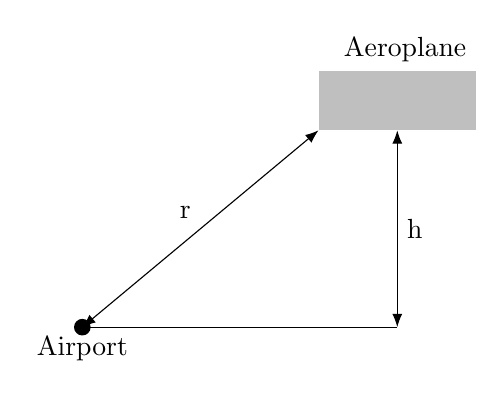
\begin{tikzpicture}
        \fill (0,0) circle (3pt) node[anchor=north] {Airport};
        \draw (0,0) -- (4,0);
        \draw[Latex-Latex] (4,0) -- (4,2.5) node[anchor=west,midway] {h};
        \draw[Latex-Latex] (0,0) -- (3,2.5) node[anchor=south east,midway] {r};
        \fill[lightgray] (3,2.5) rectangle (5,3.25) node[black,anchor=south east] {Aeroplane};
    \end{tikzpicture}
\end{figure}
This is not an orthogonal system:
\begin{align}
    \vr = (r^2-h^2)^2\hat{i} + h\hat{j}.
\end{align}
Work out the basis vectors in this coordinate system, i.e. what are $\ve_i$?
\begin{align}
    \ve_r &= \frac{\p\vr}{\p r} = \frac12 2r(r^2-h^2)^{-1/2}\hat{i} = \left(1-\frac{h^2}{r^2}\right)^{-1/2}\hat{i},\\
    \ve_h &= \frac{\p\vr}{\p h} =-\frac12 2h(r^2-h^2)^{-1/2}\hat{i} + \hat{j} = \frac{-h}{r}\left(1-\frac{h^2}{r^2}\right)^{-1/2}\hat{i}+\hat{j}.
\end{align}
What are the contravariant basis vectors, $\ve_i=\del x^i$?
We have $r^2=x^2+y^2,\,2r\frac{\p r}{\p x}=2x,\, h=y$, and then
\begin{align}
    \begin{split}
        \ve^r &= \del r = \frac{\p r}{\p x}\hat{i} + \frac{\p r}{\p y}\hat{j} = \frac{x}{r}\hat{i} + \frac{y}{r}\hat{j} \\
              &= \frac{\sqrt{r^2-h^2}}{r}\hat{i}+\frac{h}{r}\hat{j}=\left(1-\frac{h^2}{r^2}\right)^{-1/2}\hat{i}+\frac{h}{r}\hat{j},
    \end{split}\\
        \ve^h &= \del h = \frac{\p h}{\p x}\hat{i} + \frac{\p h}{\p y}\hat{j} = \hat{j}.
\end{align}

\section{Covariant and Contravariant: The Metric}
We can write vectors in either the old basis in the tangent space or the new basis in the cotangent space, i.e. $\vec{\mu}=\mu^a\ve_a=\mu_a\ve^a$.
If the basis vectors are the same, i.e. orthonormal bases, then the contravariant and covariant components are identical, but in general this is not the case. 
Take another vector, $\vec{\lambda}=\lambda^a\ve_a=\lambda_b\ve^b$.
The dot product of these is
\begin{align}
    \begin{split}
        \vec{\lambda}\cdot\vec{\mu} &= (\lambda^a\ve_a)\cdot(\mu^b\ve_b) = \lambda^a\mu^b(\ve_a\cdot\ve_b) = \lambda^a\mu^bg_{ab} \\
                                    &= |\vec{\lambda}||\vec{\mu}|\cos\chi
    \end{split}
\end{align}
Here, we use the covariant form of the metric to express the dot product of the vectors with contravariant components.
We could also express this with the covariant components, using the contravariant metric:
\begin{align}
    \vec{\lambda}\cdot\vec{\mu} &= (\lambda_a\ve^a)\cdot(\mu_b\ve^b) = \lambda_a\mu_b(\ve^a\cdot\ve^b) = \lambda_a\mu_bg^{ab}.
\end{align}
What about one with covariant and one with contravariant components?
\begin{align}
    \vec{\lambda}\cdot\vec{\mu} &= (\lambda^a\ve_a)\cdot(\mu_b\ve^b) = \lambda^a\mu_b(\ve_a\cdot\ve^b)
\end{align}
What is this dot product?
Let's do it in 3D:
\begin{align}
    \begin{split}
        \ve_i\cdot\ve^j &= \left(\frac{\p x^i}{\p x^i}\hat{i} + \frac{\p x^2}{\p x^i}\hat{j} + \frac{\p x^3}{\p x^i}\hat{k}\right)\cdot\left(\frac{\p x^j}{\p x^1}\hat{i}+\frac{\p x^j}{\p x^2}\hat{j}+\frac{\p x^j}{\p x^3}\hat{k}\right) \\
                        &= \frac{\p x^1}{\p x^i}\frac{\p x^j}{\p x^1} + \frac{\p x^2}{\p x^i}\frac{\p x^j}{\p x^2} + \frac{\p x^3}{\p x^i}\frac{\p x^j}{\p x^3} = \frac{\p x^j}{\p x^i} = \tensor{\delta}{_i^j}.
    \end{split}
\end{align}
Now because of the summation convention, $\tensor{\delta}{_i^i}=\tensor{\delta}{_1^1}+\tensor{\delta}{_2^2}+\tensor{\delta}{_3^3}=3$, so we have
\begin{align}
    (\lambda^a\ve_a)\cdot(\mu_b\ve^b) &= \lambda^a\mu_b(\ve_a\cdot\ve^b) = \lambda^a\mu_b\tensor{\delta}{^b_a} = \lambda^a\mu_a,
\end{align}
where we have contracted $\mu_b\tensor{\delta}{^b_a}$ and are now left with the repeated index to be summed over.
By symmetry of the dot product and metric, then
\begin{align}
    \lambda^a\mu_a &= \lambda_a\mu^a = g_{ab}\lambda^a\mu^b = g^{ab}\lambda_a\mu_b.
\end{align}
This gives us an easy way of swapping between contravariant and covariant components - we use the \emph{metric}:
\begin{align}
    g_{ab}\lambda^a\mu^b &= \lambda_a\mu^a, & g^{ab}\lambda_a\mu_b &= \lambda^b\mu_b, \\
    \lambda^a &= g^{ab}\lambda_b, & \lambda_a &= g_{ab}\lambda^b.
\end{align}
Tensors derived from other tensors by raising or lowering the indices via the metric are called \emph{associated tensors.}
We also get another useful metric relation in that 
\begin{align}
    \lambda_a &= g_{ab}\lambda^b = g_{ab}g^{bc}\lambda_c \implies g_{ab}g^{bc} = \tensor{\delta}{_a^c}.
\end{align}

\chapter{Derivatives in Curved Space}
We want to write normal differential equations in curved space. 
We will need:
\begin{itemize}
    \item \textbf{Parallel Transport} - derivatives in curved space are \unl{not} the same as in flat space.
    \item \textbf{Absolute Derivative} - in flat space this is the same as the normal derivative, but this is \unl{not} the case in curved space.
    \item \textbf{Covariant Derivative} - doesn't depend on the path.
\end{itemize}

\section{The Metric and Curvature of Spacetime}
Assume we deal with a space which is \emph{continuous} and \emph{differentiable}, i.e. \textbf{differentiable manifold}; also assume it has a metric. 
If the metric is positive definite (inner products are positive), then this is called a \textbf{Riemannian manifold}; if not, \textbf{pseudo-Riemannian.}
In General Relativity, there is no `force-at-a-distance' gravity anf the paths of freely-falling objects curve only because they are following the shortest path in curved spacetime (which is curved because of mass).
Any paths which follow the local curvature of spacetime (free-fall) are inertial frames, and we know how to do physics in inertial frames so we need to find what these paths are. 

\section{Parallel Transport}
In flat space, we can take a vector from a point and it keeps its direction - this is called \textbf{parallel transport.}
This is important as when we do differentials, we are comparing a vector at some point with a vector at some other point. 
In curved space, the direction the vector points at the end of the path depends on the \emph{path} as well as the start and end points. 
Consider a vector $\vec{\lambda}=\lambda^a(s)\ve_a$ defined along some curve given by coordinates $x^a(s)$, where $s$ is some point on the path. 
If we define the derivative in the `obvious' way:
\begin{align}
    \frac{d\lambda^a}{ds} &= \lim_{\delta s\to0} \left[\frac{\lambda^a(s+\delta s)-\lambda^a(s)}{\delta s}\right].
\end{align}
This does not transform, therefore it is \textbf{NOT} a tensor.
We need a tensor version to be able to use our tensor algebra. 
We want derivatives of coordinate values and how they are in the new coordinate frame:
\begin{align}
    \begin{split}
        \frac{d\lambda^{\bar{a}}}{ds} &= \frac{d}{ds}\left(\frac{\p x^{\bar{a}}}{\p x^b}\lambda^b\right) = \frac{\p x^{\bar{a}}}{\p x^b}\frac{d\lambda^b}{ds} + \lambda^b\frac{d}{ds}\left(\frac{\p x^{\bar{a}}}{\p x^b}\right),\quad \frac{d}{ds} = \frac{\p}{\p x^c}\frac{dx^c}{ds}, \\
                                      &= \underbrace{\frac{\p a^{\bar{a}}}{\p x^b}\frac{d\lambda^b}{ds}}_{\text{tensor-like}} + \lambda^b\underbrace{\left(\frac{\p^2x^{\bar{a}}}{\p x^b\p x^c}\right)}_{\text{\shortstack{change in\\ coord transforms}}}\frac{dx^c}{ds}.
    \end{split}
\end{align}
In general, the coordinate transforms such that $\frac{\p x^{\bar{a}}}{\p x^b}$ evaluated as $s+\delta s$ is not the same as $\frac{\p x^{\bar{a}}}{\p x^b}$ at $s$ as they depend on position. 
For differentiation to give a vector (tensor), we must take component differences at the same point.
In flat space, we slide one of the vectors to the other by moving one of the vectors parallel to itself, i.e. \emph{parallel transport.}
We mean that when we move the vector to its new position, it doesn't change, so
\begin{align}
    \frac{d\lambda}{ds}=0.
\end{align}
What does this parallel transport look like for a tensor?
\begin{align}
    \frac{\lambda}{ds} = 0 = \frac{d}{ds}(\lambda^a\ve_a) = \frac{d\lambda^a}{ds}\ve_a+\lambda^a\frac{d\ve_a}{ds} = \frac{d\lambda^a}{ds}\ve_a + \lambda^a\frac{\p\ve_a}{\p x^b}\frac{dx^b}{ds}.
\end{align}
We need to understand $\frac{\p\ve_a}{\p x^b}$ but since this is the derivative of a vector then it is itself a vector so we can write it as a linear combination of basis vectors:
\begin{align}
    \frac{\p\ve_a}{\p x^b} &= \tensor{\Gamma}{_{ab}^c}\ve_c,
\end{align}
where $\tensor{\Gamma}{_{ab}^c}$ are the \textbf{Christoffel Symbols,} or \emph{connection coefficients.}
We have written them in tensor notation, but they do \unl{not} transform as tensors in general. 
You can't work out the Christoffel symbols in one coordinate system and transform them into another - you have to start from the basis vectors each time. 
Christoffel symbols are a property of the spacetime in which vectors are embedded. 
\begin{align}
    \begin{split}
        \frac{d\lambda}{ds} = 0 &= \frac{d\lambda^a}{ds}\ve_a + \lambda^a\tensor{\Gamma}{_{ab}^c}\ve_c\frac{dx^b}{ds} \\
                                &= \frac{d\lambda^a}{ds}\ve_a + \lambda^b\tensor{\Gamma}{_{bc}^a}\frac{dx^c}{ds}\ve_a,
    \end{split}
\end{align}
where we relabelled indices $a\to b,\,b\to c,\,c\to a$ for the second line. 
Now we have $\ve_a$ on both terms so this is all the same vector component and we can see that, for parallel transport, we have
\begin{align}
    \frac{d\lambda^a}{ds}+\lambda^b\tensor{\Gamma}{_{bc}^a}\frac{dx^c}{ds}=0.
\end{align}
So if we parallelly-transport a vector $\lambda$ at $s$ to $s+\delta s$, we have
\begin{align}
    \frac{\delta\lambda^a}{\delta s} + \lambda^b\tensor{\Gamma}{_{bc}^a}\frac{\delta x^c}{\delta s} = 0 \implies \delta\lambda^a &= -\lambda^b\tensor{\Gamma}{_{bc}^a}\frac{\delta x^c}{\delta s}\delta s \\
    \implies \delta\lambda^a &= -\lambda^b\tensor{\Gamma}{_{bc}^a}\delta x^c = \delta\tensor{\lambda}{_{\parallel}^a}.
\end{align}
So the parallelly-transported vector has components
\begin{align}
    \lambda_{\parallel}^a(s+\delta s) = \lambda^a(s) - \lambda^b\tensor{\Gamma}{_{bc}^a}\delta x^c,
\end{align}
and we can compare this with the vector $\vec{\lambda}(s+\delta s)$ to define the \textbf{absolute derivative.}

\section{Absolute Derivative}
The point is that $\vec{\lambda}(s+\delta s)$ contains two differences with respect to $\vec{\lambda}(s)$:
\begin{itemize}
    \item Firstly, real physical differences - e.g. acceleration, deceleration, etc if the contravariant tensor is telling us about velocity.
    \item There can also be changes between these two vectors just because the \emph{space is curved.}
\end{itemize}
We want to remove these `space changes' which are what the parallelly-transported vector tells us about, so that we can see the real physical changes.
We define the absolute derivative:
\begin{align}
    \begin{split}
    \frac{D\lambda^a}{ds} &= \lim_{\delta s\to0}\left[\frac{\lambda^a(s+\delta s)-\lambda_{\parallel}^a(s+\delta s)}{\delta s}\right] \\
                          &= \frac{\left(\lambda^a(s)+\frac{d\lambda^a}{ds}\delta s\right) - \left(\lambda^a(s)+\delta\lambda_{\parallel}^a\right)}{\delta s} \\
                          &= \frac{\left(\lambda^a(s)+\frac{d\lambda^a}{ds}\delta s\right) - \left(\lambda^a(s)-\lambda^b\tensor{\Gamma}{_{bc}^a}\frac{dx^c}{ds}\delta x^c\right)}{\delta s}
    \end{split}\\
    \frac{D\lambda^a}{ds} &= \frac{d\lambda^a}{ds}+\lambda^b\tensor{\Gamma}{_{bc}^a}\frac{dx^c}{ds}.
\end{align}
Although $\frac{d\lambda^a}{ds}$ is not a tensor and $\tensor{\Gamma}{_{bc}^a}$ is not either, the two non-tensor bits cancel each other out such that $\frac{D\lambda^a}{ds}$ \unl{does} transform as a tensor. 
So to define the physical, or \textbf{absolute derivative}, we use parallel transport to take out the space changes. 
We are left with a value which is \emph{independent of coordinate system} but does depend on the path taken, i.e. \textbf{path dependent.}

\section{Covariant Derivative}
We can do this in terms of coordinates as opposed to a single parameter, and remove the path dependence. 
Writing the absolute derivative with a partial in the first term:
\begin{align}
    \frac{D\lambda^a}{ds} &= \frac{\p\lambda^a}{\p x^c}\frac{dx^c}{ds} + \lambda^b\tensor{\Gamma}{_{bc}^a}\frac{dx^c}{ds} = \left(\frac{\p\lambda^a}{\p x^c} + \tensor{\Gamma}{^a_{bc}}\lambda^b\right)\frac{dx^c}{ds} = \tensor{\lambda}{^a_{;c}}\frac{dx^c}{ds}
\end{align}
So the components of the \textbf{covariant derivative} are
\begin{align}
    \tensor{\lambda}{^a_{;c}} &\equiv \del_c\lambda^a = \frac{\p\lambda^a}{\p x^c}+\tensor{\Gamma}{^a_{bc}}\lambda^b
\end{align}
You can check this notation; note this is a derivative. 
This is closely related to the absolute derivative, which is a Rank (0,1) tensor, so this is a Rank (1,1) tensor. 

\section{The Christoffel Symbols}
What are these $\tensor{\Gamma}{^a_{bc}}$?
They come from the derivatives of the tangent basis vectors, but these are defined $\ve_a=\frac{\p\vr}{\p x^a}$, so
\begin{align}
    \tensor{\Gamma}{_{ab}^c}\ve_c &= \frac{\p\ve_a}{\p x^b} = \frac{\p^2\vr}{\p x^a\p x^b} = \frac{\p^2\vr}{\p x^b\p x^a} = \frac{\p\ve_b}{\p x^a} = \tensor{\Gamma}{_{ba}^c}\ve_c.
\end{align}
They are symmetric, (changing the order of integration assumes that the second partial derivatives are continuous) so we only need half as many Christoffel symbols as initially thought since $\tensor{\Gamma}{_{ab}^c}=\tensor{\Gamma}{_{ba}^c}$.\\
We can also look at how the metric changes as a function of the coordinates:
\begin{align}
    \begin{split}
        \frac{\p}{\p x^c}(g_{ab}) &= \frac{\p}{\p x}(\ve_a\cdot\ve_b) + \frac{\p\ve_a}{\p x^c}\cdot\ve_b + \ve_a\cdot\frac{\p\ve_b}{\p x^c} \\
                                  &= (\tensor{\Gamma}{_{ac}^d}\ve_d)\cdot\ve_b+\ve_a\cdot(\tensor{\Gamma}{_{bc}^d}\ve_d),
    \end{split}\\
    \frac{\p}{\p x^c}(g_{ab}) &= \tensor{\Gamma}{_{ac}^d}g_{db} + \tensor{\Gamma}{_{bc}^d}g_{ad},\\
    \frac{\p}{\p x^a}(g_{bc}) &= \tensor{\Gamma}{_{ba}^d}g_{dc} + \tensor{\Gamma}{_{ca}^d}g_{bd},\\
    \frac{\p}{\p x^b}(g_{ca}) &= \tensor{\Gamma}{_{cb}^d}g_{da} + \tensor{\Gamma}{_{ab}^d}g_{cd},
\end{align}
If we add the first two and subtract the third, we get an expression for the Christoffel symbols in terms of the derivatives of the metric:
\begin{align}
    \frac{\p g_{ab}}{\p x^c} + \frac{\p g_{bc}}{\p x^a} - \frac{\p g_{ca}}{\p x^b} = 2\tensor{\Gamma}{_{ca}^d}g_{db}.
\end{align}
Multiplying by $\frac12 g^{fb}$ and remembering that $g^{fb}g_{db} = \tensor{\delta}{^f_d}$, we get
\begin{align}
    \tensor{\Gamma}{_{ca}^f} = \frac12g^{fb}\left(\frac{\p g_{bc}}{\p x^a} - \frac{\p g_{ca}}{\p x^b} + \frac{\p g_{ab}}{\p x^c}\right).
\end{align}
Using the notation $\frac{\p}{\p x^c}\equiv\p_c$ and the symmetry $\tensor{\Gamma}{_{ca}^f}=\tensor{\Gamma}{_{ac}^f}$ yields
\begin{align}
    \tensor{\Gamma}{_{ac}^f} = \frac12g^{fb}\left(\p_ag_{bc}-\p_bg_{ca}+\p_cg_{ab}\right).
\end{align}
So if we have a metric (and time), we can calculate these, since we can calculate derivatives of the metric. 

\textbf{Notation:}
\begin{itemize}
    \item \textbf{Partial Derivative:} $\frac{\p A^a}{\p x^c} = \p_cA^a = \tensor{A}{^a_{;c}}$
    \item \textbf{Covariant Derivative:} $\del_cA^a=\tensor{A}{^a_{;c}}$
    \item \textbf{Absolute Derivative:} $\del_{\bar{u}}A^a = \frac{DA^a}{ds}$
    \item \textbf{Christoffel Symbols:} $\tensor{\Gamma}{_{bc}^a}$ or $\{\frac{a}{bc}\}$ or $\{a,bc\}$
\end{itemize}

\chapter{Calculating Christoffel Symbols}
\begin{example}[2D flat space]
The metric for flat space in Cartesian coordinates $x^A = \{x,y\}$, $g_{AB} = \text{diag}(1,1) = \begin{pmatrix} 1 & 0 \\ 0 & 1 \end{pmatrix}$ doesn't depend on position so the partial derivatives of the metric are zero, i.e. $\tensor{\Gamma}{^A_{BC}} = 0$.
This is not true if we use \emph{polars}:
\begin{align}
    ds^2 &= dr^2 + r^2\,d\theta^2 \\
    g_{AB} &= \text{diag}(1,r^2) \\
    \tensor{\Gamma}{^A_{BC}} &\neq 0
\end{align}
So the Christoffel symbols tell us about the curvature, but also about the coordinate system we have chosen, i.e. non-zero in flat 2D from changing coordinate system. 
\end{example}

\begin{example}[Surface of a Sphere]
In 3D space, we have
\begin{align}
    ds^2 &= dr^2 + r^2\,d\theta^2 + r^2\sin^2\theta\,d\phi^2
\end{align}
and we can limit this at a fixed radius $r=a$ so $dr=0$ for 2D, so
\begin{align}
    ds^2 &= a^2\,d\theta^2 + a^2\sin^2\theta\,d\phi^2 = g_{AB}dx^A\,dx^B \\
    g_{AB} &= \text{diag}(a^2,a^2\sin^2\theta)
\end{align}
The Christoffel symbols are defined as
\begin{align}
    \tensor{\Gamma}{_{AC}^F} &= \frac12g^{FB}\left(\p_Ag_{BC}-\p_Bg_{CA}+\p_Cg_{AB}\right),
\end{align}
so we also need the \emph{covariant metric components} $g^{AB}$ from
\begin{align}
    g^{AB}g_{BC} &= \tensor{\delta}{^A_C}.
\end{align}
In general, this leads to a set of simultaneous equations to solve:
\begin{align}
    g^{AB}g_{BC} = g^{A1}g_{1C} + g^{A2}g_{2C} = \tensor{\delta}{^A_C}.
\end{align}
For diagonal \textbf{only}, we don't have to do a matrix inverse to solve these as all cross-terms are zero, so we get
\begin{align}
    g^{AB}g_{BA} &= g^{AA}g_{AA} = 1 \implies g^{AA} = \frac{1}{g_{AA}}.
\end{align}
If the covariant form of the metric is diagonal, then so is the \emph{contravariant metric}.
So we have
\begin{align}
    g^{AB} &= \text{diag}\left(\frac{1}{a^2},\frac{1}{a^2\sin^2\theta}\right)
\end{align}
So in our 2D space, we have
\begin{align}
    \tensor{\Gamma}{^\theta_{\theta\theta}} &= \frac12 g^{\theta B} \left(\p_\theta g_{B\theta} - \p_B g_{\theta\theta} + \p_{\theta} g_{\theta B}\right), \quad g^{\theta B} = 0, B\neq\theta,
\end{align}
and as $g^{\theta B}=0$ except for when $B=\theta$, this then collapses to
\begin{align}
    \tensor{\Gamma}{^\theta_{\theta\theta}} &= \frac12 g^{\theta\theta}\left(\p_\theta\cancel{g_{\theta\theta}}-\p_\theta\cancel{g_{\theta\theta}}+\p_\theta\cancel{g_{\theta\theta}}\right) = \frac12\cdot \frac{1}{a^2} \cdot 0 = 0.
\end{align}
The bracket terms are all zero as $g_{\theta\theta}=a^2$ is not proportional to $\theta$ and so the partial with repsect to $\theta$ is zero.
\begin{align}
    \tensor{\Gamma}{^\theta_{\phi\theta}} = \tensor{\Gamma}{^\theta_{\theta\phi}} &= \frac12 g^{\theta B}\left(\p_\theta g_{B\phi} - \p_B g_{\phi\theta} + \p_\phi g_{\theta B}\right),
\end{align}
where again $g^{\theta B}$ is only non-zero for $B=\theta$ since the metric is diagonal, so:
\begin{align}
    \tensor{\Gamma}{^\theta_{\phi\theta}} = \tensor{\Gamma}{^\theta_{\theta\phi}} &= \frac12 g^{\theta\theta}\left(\p_\theta \cancel{g_{\theta\phi}} - \p_\theta \cancel{g_{\phi\theta}} + \p_\phi \cancel{g_{\theta\theta}}\right) = \frac12\cdot\frac{1}{a^2}\cdot0 = 0, \\
    \tensor{\Gamma}{^\theta_{\phi\phi}} &= -\sin\theta\cos\theta, \\
    \tensor{\Gamma}{^\phi_{\theta\phi}} &= \cot\theta.
\end{align}
The rest of the Christoffel symbols for this example are 0 (there are $2^3=8$ in total).
\end{example}

\section{Geodesic Equations}
We have everything we need to get \textbf{geodesic paths} (inertial frames).
In maths, they define geodesics as the shortest distance between two points. 
In physics, these are inertial frames and in an inertial frame the velocity doesn't change. 
There are \emph{no forces to produce an acceleration.}
We define velocity as a tensor as
\begin{align}
    \vec{v} &= v^\alpha\ve_{\alpha} = \frac{\p x^\alpha}{\p\tau}\ve_\alpha.
\end{align}
If there is no change in this, then its derivative is zero, but we also saw that there can be swings in a vector which arise from curved space. 
We say its the \emph{absolute derivative} which is zero:
\begin{align}
    \frac{Dv^\alpha}{d\tau} &= 0
\end{align}
By an affine parameter, we mean a linear function of path length $u=A+Bs$, such as the proper time $\tau$, so the components change like
\begin{align}
    \frac{dv^\alpha}{d\tau} + \tensor{\Gamma}{^\alpha_{\beta\gamma}}v^\beta\frac{dx^\gamma}{d\tau} &= 0, \\
    \frac{d^2x^\alpha}{d\tau^2} + \tensor{\Gamma}{^\alpha_{\beta\gamma}}\frac{dx^\beta}{d\tau}\frac{dx^\gamma}{d\tau} &= 0,
\end{align}
and we can use the notation where a dot means derivative with respect to time to write this as
\begin{align}
    \ddot{x}^\alpha + \tensor{\Gamma}{^\alpha_{\beta\gamma}}\dot{x}^\beta\dot{x}^\gamma &= 0.
\end{align}
This works for any parameter linearly-related to path length $s$, i.e. for $u=A+Bs$ or $\tau=\frac{1}{c}s$, our \emph{affine parameters.}
This is the \emph{affinely-parameterised geodesic equation} in an N-dimensional manifold.
Although this is a second-order differential equation, we cannot just integrate due to the summations.
\begin{example}[Geodesics in Flat Space]
In flat space, all $\tensor{\Gamma}{^i_{jk}}=0$ so the geodesic equations become $\ddot{x}^a = 0$, where dot denotes derivatives with respect to path length $s$.
We integrate to get $\dot{x}^a=A$ and $x^a=As+B$, so geodesics in flat space have constant velocity and direction - \emph{Newtonian inertial frames.}
\end{example}
\begin{example}[Geodesics on a Sphere - Paths in $\theta$]
In general, it is too difficult to do geodesics in full generality - often, we just choose a path and see if its a geodesic. 
A natural choice is a path defined by only one of the parameters, called a \emph{parameter curve.}
We know that for a sphere the only non-zero Christoffel symbols are
\begin{align}
    \tensor{\Gamma}{^\theta_{\phi\phi}} &= -\sin\theta\cos\theta, & \tensor{\Gamma}{^\phi_{\theta\phi}} &= \tensor{\Gamma}{^\phi_{\phi\theta}} = \cot\theta.
\end{align}
Geodesic paths satisfy the equation
\begin{align}
    \frac{d^2x^A}{ds^2} + \tensor{\Gamma}{^A_{BC}}\frac{dx^B}{ds}\frac{dx^c}{ds} = 0.
\end{align}
Suppose the path $s$ is just a change in $\theta$, then $s=a\theta$, so there is no dependence on $\phi$, i.e. $x^2=\phi=$ constant$\implies\frac{d\phi}{ds}=0$, while for $\theta$ we have 
\begin{align}
    \theta &= \frac{s}{a},\quad \frac{d\theta}{ds} = \frac{1}{a},\quad \frac{d^2\theta}{ds^2} = 0,\\
    \frac{d^2\theta}{ds^2} &+ \tensor{\Gamma}{^\theta_{BC}}\frac{dx^B}{ds}\frac{dx^c}{ds} = \frac{d^\theta}{ds^2} + \tensor{\Gamma}{^\theta_{\phi\phi}}\frac{d\phi}{ds}\frac{d\phi}{ds} = 0.
\end{align}
This satisfies the geodesic equation in $\theta$, so we get a big tick and a gold star!
We should check that this also holds in $\phi$:
\begin{align}
    \frac{d^2\phi}{ds^2} + \tensor{\Gamma}{^\phi_{BC}}\frac{dx^B}{ds}\frac{dx^C}{ds} = \frac{d^2\phi}{ds^2} + \tensor{\Gamma}{^\phi_{\theta\phi}}\frac{d\theta}{ds}\frac{d\phi}{ds} + \tensor{\Gamma}{^\phi_{\phi\theta}}\frac{d\phi}{ds}\frac{d\theta}{ds} = 0
\end{align}
So it's a geodesic path! Yayyyyyy!
\end{example}
\begin{example}[Geodesics on a Sphere - Paths in $\phi$]
Suppose the path $s$ is just a change in $\phi$, then $s=a\phi$ so there is no dependence on $\theta$, i.e. 
\begin{align}
    x^\theta &= \theta_0, & \frac{d\theta}{ds} &= 0, & \frac{d^2\theta}{ds^2} &= 0,\\
    \phi &= \frac{s}{a}, & \frac{d\phi}{ds} &= \frac1a, & \frac{d^2\phi}{ds^2} &= 0.
\end{align}
The LHS of the geodesic equation in $\phi$ is then
\begin{align}
    \frac{d^\phi}{ds^2} + \tensor{\Gamma}{^\phi_{BC}}\frac{dx^B}{ds}\frac{dx^C}{ds} = 0 + \tensor{\Gamma}{^\phi_{\theta\phi}}\frac{d\theta}{ds}\frac{d\phi}{ds} + \tensor{\Gamma}{^\phi_{\phi\theta}}\frac{d\phi}{ds}\frac{d\theta}{ds} = 0,
\end{align}
and the LHS of the geodesic equatoin in $\theta$ is 
\begin{align}
    \frac{d^2\theta}{ds^2} + \tensor{\Gamma}{^\theta_{BC}}\frac{dx^B}{ds}\frac{dx^C}{ds}=\frac{d^2\theta}{ds^2}+\tensor{\Gamma}{^\theta_{\phi\phi}}\frac{d\phi}{ds}\frac{d\phi}{ds} = 0 - \sin\theta_0\cos\theta_0\frac1a.
\end{align}
This is only equal to zero (i.e. only a geodesic) for the special case of $\sin\theta_0\cos\theta_0=0\to\theta_0=0,\frac{\pi}{2},\pi$.
$0,\pi$ are the N and S poles respectively where a path in $\phi$ is just a point. 
The only geodesics which involve any distance is the equator. 
\end{example}

\chapter{Easier Christoffel Symbols and Geodesics Paths}
\section{Euler-Lagrange Equations}
An easier way to find Christoffel symbols and geodesic paths is to use the \emph{Euler-Lagrange equations.}
We could have solved for the \emph{geodesics} by saying that these are the paths which give the shortest distance between two points, i.e. we are looking for the external path which has
\begin{align}
    \delta\left[\int ds\right] = 0.
\end{align}
The shortest path is a minimum. 
This is often what we do in \emph{classical mechanics} where we look for the minimum energy path by getting the \emph{Lagrangian} $L=T-V$, as the sum of the kinetic $T$ and potential $V$ energies, and then finding the minimum energy path by integrating this over time, i.e.
\begin{align}
    \delta\left[\int \La\,dt\right] = 0.
\end{align}
For \emph{freely-moving particles} (i.e. those on geodesics), there are no potential energy terms as $V=0$, so we are only looking at the kinetic energy:
\begin{align}
    \delta\left[\int \La\,dt\right] = \delta\left[\int T\,dt\right] = 0.
\end{align}
In terms of per unit mass,
\begin{align}
    T &= \frac12\left[\left(\frac{dx}{dt}\right)^2 + \left(\frac{dy}{dt}\right)^2 + \left(\frac{dz}{dt}\right)^2\right],
\end{align}
or in terms of the \emph{metric} (in Euclidean 3D non-relativistic flat space),
\begin{align}
    T &= \frac12g_{ij}\frac{dx^i}{dt}\frac{dx^j}{dt} = \frac12g_{ij}\dot{x}^i\dot{x}^j = \frac12\left(\frac{ds}{dt}\right)^2.
\end{align}
So the \emph{minimum energy condition} (Hamilton's principle in classical mechanics) gives
\begin{align}
    \delta\left[\int T\,dt\right] &= \delta\left[\int \left(\frac{ds}{dt}\right)^2\,dt\right] = 0,
\end{align} 
i.e. this is basically the same as the minimum path requirement which defines our geodesic path which is 
\begin{align}
    \delta\left[\int \left(\frac{ds}{dt}\right)\,dt\right] = 0.
\end{align}
We know that in classical mechanics the solution with the minimum energy satisfies the \emph{Euler-Lagrange equations,} i.e.
\begin{align}
    \dt\left(\frac{\p\La}{\p\dot{x}^i}\right) - \frac{\p\La}{\p x^i} &= 0, & \La &= \frac12g_{ij}\dot{x}^i\dot{x}^j.
\end{align}
There are some technical problems using this in 4D spacetime, where the metric is indefinite (it can be positive, negative, or zero); if you do it, then it comes out to be the same except we now take our derivative with respect to some \emph{affine parameter}, linearly related to the \emph{invariant path length, s} rather than to t.
So the dots then stand for the derivative with respect to the affine parameter, e.g. \emph{geodesic paths} are now
\begin{align}
    \ddot{x}^\alpha + \tensor{\Gamma}{^\alpha_{\beta\gamma}}\dot{x}^\beta\dot{x}^\gamma &= 0.
\end{align}
Classically, we used $\dt$, now in relativity we use $\frac{d}{ds}$ (which is pretty much equivalent to $c\dt$) and/or $\frac{d}{d\tau}$.
We could use any affine parameter, but we will use $\tau=\frac{s}{c}$ here. 
So we now have the \emph{Euler-Lagrange equation} as
\begin{align}
    \frac{d}{ds}\left(\frac{\p\La}{\p\dot{x}^b}\right) - \frac{\p\La}{\p x^b} &= 0, & \La &= \frac12g_{ab}\dot{x}^a\dot{x}^b.
\end{align}
From these, we can return an equation similar to the geodesic equation from which we can get the Christoffel symbols. 

\section{Equivalence of the Geodesic and Euler-Lagrange Equations}
We frequently change the letters as we want here, so \textbf{be careful.}
We write the \emph{geodesic equation} as
\begin{align}
    \ddot{x}^f + \tensor{\Gamma}{^f_{ac}}\dot{x}^a\dot{x}^c &= 0.
\end{align}
This will be helpful for later. 
The Christoffel symbols are defined as usual as
\begin{align}
    \tensor{\Gamma}{^f_{ac}} &= \frac12g^{fb}\left(\p_ag_{bc}-\p_bg_{ca}+\p_cg_{av}\right). 
\end{align}
Using the Euler-Lagrange equation and the Lagrangian as
\begin{align}
    \frac{d}{ds}\left(\frac{\p\La}{\p\dot{x}^c}\right) - \frac{\p\La}{\p x^c} &= 0, & \La &= \frac12g_{ac}\dot{x}^a\dot{x}^c,
\end{align}
noting notation and that $g_{ab}$ is a metric which only depends on position, i.e. $x^c$, and not velocity, i.e. $\dot{x}^c$.
Doing the substitution, we get
\begin{align}
    \frac{\p\La}{\p\dot{x}^b} &= \frac{\p}{\p\dot{x}^b}\left(\frac12g_{ab}\dot{x}^a\dot{x}^c\right) = \frac12\dot{x}^a\dot{x}^c\frac{\p g_{ac}}{\p\dot{x}^b} + \frac12g_{ac}\overbrace{\frac{\p\dot{x}^a}{\p\dot{x}^b}}^{\delta^a_b}\dot{x}^a + \frac12g_{ac}\dot{x}^a\overbrace{\frac{\p\dot{x}^c}{\p\dot{x}^b}}^{\delta^c_b},
\end{align}
and as mentioned above $\frac{\p}{\p\dot{x}^b}g_{ac}=0$, so
\begin{align}
    0 + \frac12g_{ac}\dot{x}^c\tensor{\delta}{^a_b}+\frac12g_{ac}\dot{x}^a\tensor{\delta}{^c_b} &= \frac12g_{ab}\dot{x}^a+\frac12g_{bc}\dot{x}^c,
\end{align} 
and changing $c\to a$ and $g_{ab}=g_{ba}$, and then $a\to e$, 
\begin{align}
    \frac12g_{ab}\dot{x}^a+\frac12g_{ab}\dot{x}^a &= g_{be}\dot{x}^e.
\end{align}
Into the Euler-Lagrange equation:
\begin{align}
    \frac{d(a^2\dot{\theta})}{ds} - a^2\dot{\phi}^2\sin\theta\cos\theta &= 0, \\
    \cancel{a^2}\ddot{\theta} - \cancel{a^2}\dot{\phi}^2\sin\theta\cos\theta &= 0,
\end{align}
which we compare with the equivalent geodesic equation,
\begin{equation}
    \ddot{\theta} + \tensor{\Gamma}{^\theta_{BC}}\dot{x}^B\dot{x}^C = 0,
\end{equation}
and expanding the double sum:
\begin{align}
    \ddot{\theta} + \tensor{\Gamma}{^\theta_{\theta\theta}}\dot{\theta}\dot{\theta} + \tensor{\Gamma}{^\theta_{\phi\theta}}\dot{\phi}\dot{\theta} + \tensor{\Gamma}{^\theta_{\theta\phi}}\dot{\theta}\dot{\phi} + \tensor{\Gamma}{^\theta_{\phi\phi}}\dot{\phi}\dot{\phi} = 0.
\end{align}
Equating coefficients and see that $\tensor{\Gamma}{^\theta_{\theta\theta}}=\tensor{\Gamma}{^\theta_{\phi\theta}}=\tensor{\Gamma}{^\theta_{\theta\phi}}=0$, but $\tensor{\Gamma}{^\theta_{\phi\phi}}=-\sin\theta\cos\theta$ as we have $\dot{\phi}^2$.
For $\phi$, we then have
\begin{align}
    \frac{\p\La}{\p\dot{\phi}} = a^2\sin^2\theta\dot{\phi},\qquad \frac{\p\La}{\p\phi} &= 0,\qquad \frac{d}{ds}(a^2\sin^2\theta\dot{\phi})-0 = 0, \\
    \frac{d}{ds}\left(\frac{\p\La}{\p\dot{\phi}}\right) - \frac{\p\La}{\p\phi} &= 0,\\
    \begin{split}
        \frac{\p}{\p\theta}(\sin^2\theta)\frac{d\theta}{ds}\dot{\phi} + \sin^2\ddot{\phi} &= 0, \\
        2\cos\theta\sin\theta\dot{\theta}\dot{\phi} + \sin^2\theta\ddot{\phi} &= 0,\\
        2\cos\theta\dot{\theta}\dot{\phi} + \sin\theta\ddot{\phi} &= 0, \\
        \ddot{\phi} + 2\left(\frac{\cos\theta}{\sin\theta}\right)\dot{\theta}\dot{\phi} &= 0,
    \end{split}\\
    \ddot{\phi} + 2\cot\theta\dot{\theta}\dot{\phi} &= 0.
\end{align}
Compare this with the geodesic equation in $\phi$:
\begin{align}
    \ddot{\phi} + \tensor{\Gamma}{^\phi_{\theta\theta}}\dot{\theta}\dot{\theta} + 2\tensor{\Gamma}{^\phi_{\theta\phi}}\dot{\theta}\dot{\phi} + \tensor{\Gamma}{^\phi_{\phi\phi}}\dot{\phi}\dot{\phi} &= 0.
\end{align}
Then, equating the coefficients, we get $\tensor{\Gamma}{^\phi_{\phi\phi}} = \tensor{\Gamma}{^\phi_{\theta\theta}} = 0$, but $2\tensor{\Gamma}{^\phi_{\theta\phi}} = 2\cot\theta$, so we can conclude with
\begin{align}
    \tensor{\Gamma}{^\phi_{\theta\phi}} &= \cot\theta.
\end{align}
Christoffel symbols tell you about the coordinate system and the curvature of space, i.e. whether space is curved or not. 

\chapter{More Tensor Derivatives}
The absolute derivative of a \emph{contravariant tensor} over some path,
\begin{align}
    \frac{D\lambda^a}{ds} &=\frac{d\lambda^a}{ds} +\tensor{\Gamma}{^a_{bc}}\lambda^b\frac{dx^c}{ds},
\end{align}
gives a tensor field of the same type.
The first term takes into account both physical (real) changes in $\lambda^a$ and the way the curvature of the space can swimg the vector; the second term takes out the swinging of the vector from the curvature of space alone.
If there is no physical change, then the vector is simply \emph{parallelly-transported} and
\begin{align}
    \frac{D\lambda^a}{ds} = 0.
\end{align}
The \emph{absolute derivative} obeys all the normal rules for derivatives so we have:
\begin{enumerate}
    \item The derivative is a \emph{linear operation}:
        \begin{align}
            \frac{D}{ds}\left(\lambda^a+ k\mu^a\right) = \frac{D\lambda^a}{ds} + k\frac{D\mu^a}{ds}.
        \end{align}
    \item The Leibniz chain rule:
        \begin{align}
            \frac{D}{ds}\left(\lambda^a\mu^b\right) = \mu^b\frac{D\lambda^a}{ds} + \lambda^a\frac{D\mu^b}{ds}.
        \end{align}
\end{enumerate}

\section{The Absolute Derivative of a Scalar}
$\phi$, a scalar, the number of which varies according to where it is in space, but it \emph{does not depend on the coordinate system} (as tensors do), so we have
\begin{align}
    \frac{D\phi}{ds} = \frac{d\phi}{ds}.
\end{align}
This is the \textbf{Scalar Absolute Derivative} and is like a normal derivative.

\section{The Absolute Derivative of Covariant Tensors}
We have defined the absolute derivative of a contravariant tensor, but now what about a covariant tensor $\mu_a$?
We can write a scalar as $\phi=\lambda^a\mu_a$, for which we have the above, $\frac{D\phi}{ds} = \frac{d\phi}{ds}$, then
\begin{align}
    \frac{D\phi}{ds} &= \frac{D}{ds}(\lambda^a\mu_a) = \mu_a\frac{D\lambda^a}{ds}+\lambda^a\frac{D\mu_a}{ds}, 
\end{align}
and we have the absolute derivative of $\lambda^a$:
\begin{align}
    \frac{D\lambda^a}{ds} &= \frac{d\lambda^a}{ds} + \tensor{\Gamma}{^a_{bc}}\lambda^b\frac{dx^c}{ds},
    \implies \frac{d\phi}{ds} = \mu_a\left(\frac{d\lambda^a}{ds} + \tensor{\Gamma}{^a_{bc}}\lambda^b\frac{dx^c}{ds}\right) + \lambda^a\frac{D\mu_a}{ds},
\end{align}
and then using the chain rule for $\frac{d\phi}{ds}$:
\begin{align}
    \frac{d\phi}{ds} &= \frac{d}{ds}(\lambda^a\mu_a) = \mu_a\frac{d\lambda^a}{ds}+\lambda^a\frac{d\mu_a}{ds}, \\
    \lambda^a\frac{d\mu_a}{ds} + \cancel{\mu_a\frac{d\lambda^a}{ds}} &= \cancel{\mu_a\frac{d\lambda^a}{ds}} + \mu_a\lambda^b\tensor{\Gamma}{^a_{bc}}\frac{dx^c}{ds} + \lambda^a\frac{D\mu_a}{ds},\\
    \begin{split}
        \lambda^a\frac{d\mu_a}{ds} &= \mu_a\tensor{\Gamma}{^a_{bc}}\lambda^b\frac{dx^c}{ds} + \lambda^a\frac{D\mu_a}{ds}, \\
                                   &= \mu_b\tensor{\Gamma}{^b_{ac}}\lambda^a\frac{dx^c}{ds} + \lambda^a\frac{D\mu_a}{ds}.
    \end{split}
\end{align}
We now have an expression with $\lambda^a$ in all terms and as it is a tensor, this must be true for any $\lambda^a$ if the other parts are true. 
We can then `cancel' $\lambda^a$ through unity, as the remaining equation must also be true:
\begin{align}
    \frac{d\mu_a}{ds} &= \tensor{\Gamma}{^b_{ac}}\mu_b\frac{dx^c}{ds} + \frac{D\mu_a}{ds}.
\end{align}
So rearranging gives us the \textbf{Absolute Derivative of Covariant Tensors}:
\begin{align}
    \frac{D\mu_a}{ds} &= \frac{d\mu_a}{ds} - \tensor{\Gamma}{^b_{ac}}\mu_b\frac{dx^c}{ds}.
\end{align}

\section{The Absolute Derivative of Higher-Order Tensors}
What is the absolute derivative of a rank (1,1) tensor, e.g. $\tensor{\tau}{^a_b}=\lambda^a\mu_b$?
\begin{align}
    \begin{split}
        \frac{D\tensor{\tau}{^a_b}}{ds} &= \frac{D(\lambda^a\mu_b)}{ds} = \mu_b\frac{D\lambda^a}{ds} + \lambda^a\frac{D\mu_b}{ds}, \\
                                        &= \mu_b\left[\frac{d\lambda^a}{ds}+\tensor{\Gamma}{^a_{dc}}\lambda^d\frac{dx^c}{ds}\right] + \lambda^a\left[\frac{d\mu_b}{ds}-\tensor{\Gamma}{^d_{bc}}\mu_d\frac{dx^c}{ds}\right],\\
                                        &= \frac{d}{ds}(\lambda^a\mu_b) + \mu_b\tensor{\Gamma}{^a_{dc}}\lambda^a\frac{dx^c}{ds} - \lambda^a\tensor{\Gamma}{^d_{bc}}\mu_d\frac{dx^c}{ds},\\
                                        &= \frac{d}{ds}(\tensor{\tau}{^a_b}) + \tensor{\Gamma}{^a_{dc}}\tensor{\tau}{^d_b}\frac{dx^c}{ds} - \tensor{\Gamma}{^d_{bc}}\tensor{\tau}{_d^a}\frac{dx^c}{ds}.
    \end{split}
\end{align}
We could also do this to, for example, $\tensor{R}{^a_{bcd}}$ (Riemann's curvature tensor) which we will use later.

\section{Covariant Derivative}
What about the covariant derivative?
It is defined as
\begin{align}
    \tensor{\lambda}{^a_{;c}} &= \frac{\p\lambda^a}{\p x^c} + \tensor{\Gamma}{^a_{bc}}\lambda^b.
\end{align}
This is like the partial derivative in curved spacetime. 
It is related to the absolute derivative as
\begin{align}
    \begin{split}
        \frac{D\lambda^a}{ds} &= \tensor{\lambda}{^a_{;c}}\frac{dx^c}{ds} = \frac{\p\lambda^a}{\p x^c}\frac{dx^c}{ds} + \tensor{\Gamma}{^a_{bc}}\lambda^b\frac{dx^c}{ds}\\
                              &= \frac{d\lambda^a}{ds} + \tensor{\Gamma}{^a_{bc}}\lambda^b\frac{dx^c}{ds}.
    \end{split},
\end{align}
so we've brought ourselves back to the absolute derivative. 
The rules as before carry over again, so we can now write out the covariant derivative for a second-order contravariant tensor:
\begin{align}
    \begin{split}
        \tensor{\tau}{^{ab}_{;c}} &= (\lambda^a\mu^b)_{;c} = \tensor{\lambda}{^a_{;c}}\mu^b + \lambda^a\tensor{\mu}{^b_{;c}} \\
                                  &= \frac{\p\lambda^a}{\p x^c}\mu^b + \tensor{\Gamma}{^a_{dc}}\lambda^d\mu^b + \lambda^a\frac{\p\mu^b}{\p x^c} + \lambda^a\tensor{\Gamma}{^b_{dc}}\mu^d \\
                                  &= \p_c\tau^{ab} + \tensor{\Gamma}{^a_{dc}}\tau^{db} + \tensor{\Gamma}{^d_{ac}}\tau^{ad}
    \end{split}
\end{align}
For the covariant derivative of a scalar, we have
\begin{align}
    \phi_{;c} &= \frac{\p\phi}{\p x^c} = \p_c\phi,
\end{align}
which is the same as the partial derivative of the scalar. 
Let $\phi=\lambda^a\mu_a$, and we can find the \emph{covariant derivative of a covariant tensor}:
\begin{align}
    \begin{split}
        \phi_{;c} = \p_c\phi &= (\lambda^a\mu_a)_{;c} = (\tensor{\lambda}{^a_{;c}})\mu_a + \lambda^a(\mu_{a;c}), \\
        \frac{\p\phi}{\p x^c} &= \cancel{\left(\frac{\p\lambda^a}{\p x^c}\right)}\mu_a + \lambda^a\left(\frac{\p\mu_a}{\p x^c}\right) = \left(\cancel{\frac{\p\lambda^a}{\p x^c}} + \tensor{\Gamma}{^a_{dc}}\lambda^d\right)\mu_a + \lambda^a\mu_{a;c} 
    \end{split}\\
    \lambda^a\frac{\p\mu_a}{\p x^c} &= \tensor{\Gamma}{^a_{dc}}\lambda^d\mu_a + \lambda^a\mu_{a;c}
\end{align}
and relabelling indices to get all $\lambda$ compenents to $\lambda^a$,
\begin{align}
    \lambda^a\frac{\p\mu_a}{\p x^c} &= \tensor{\Gamma}{^b_{ac}}\lambda^a\mu_b +\lambda^a\mu_{a;c},\\
    \mu_{a;c} &= \frac{\p\mu_a}{\p x^c}-\tensor{\Gamma}{^b_{ac}}\mu_b,
\end{align}
and so we have our \textbf{Covariant Derivative of a Covariant Tensor.}
We can do higher-order covariant derivatives similarly, yielding
\begin{align}
    \lambda_{ab;c} &= \frac{\p\lambda_{ab}}{\p x^c} - \tensor{\Gamma}{^d_{ac}}\lambda_{db}-\tensor{\Gamma}{^d_{bc}}\lambda_{ad}.
\end{align}
Covariant differentiation forms a tensor field of one higher covariant order than the original tensor field.

\section{Covariant Derivative of the Metric}
In getting the Christoffel symbols in terms of the metric, we had
\begin{align}
    \begin{split}
    \frac{\p g_{ab}}{\p x^c} &= \frac{\p}{\p x^c} (\ve_a\cdot\ve_b) = \frac{\p\ve_a}{\p x^c}\cdot\ve_b + \ve_a\cdot\frac{\p\ve_b}{\p x^c},\\
                             &= \left(\tensor{\Gamma}{^d_{ac}}\ve_d\right)\cdot\ve_b + \ve_a\cdot\left(\tensor{\Gamma}{^d_{bc}}\ve_d\right) = \tensor{\Gamma}{^d_{ac}}g_{db} + \tensor{\Gamma}{^d_{bc}}g_{ad},
    \end{split}\\
    \frac{\p g_{ab}}{\p x^c} &- \tensor{\Gamma}{^d_{ac}}g_{db} - \tensor{\Gamma}{^d_{bc}}g_{ad} = 0,
\end{align}
Comparing this to the definition of the covariant of a second-order covariant tensor, this is
\begin{align}
    g_{ab;c} = 0,
\end{align}
and we can similarly get
\begin{align}
    \tensor{g}{^{ab}_{;c}} = 0.
\end{align}
This means that index lowering can be swapped in and out of covariant differentiation. 
Why is this important?
The metric allows us to switch coordinate systems as
\begin{align}
    R_a &= g_{ab}R^b,\qquad R_{a;c} = (g_{ab}R^b)_{;c},\\
    R_{a;c} &= \cancel{g_{ab;c}R^b} + g_{ab}\tensor{R}{^b_{;c}} = g_{ab}\tensor{R}{^b_{;c}}.
\end{align}
Likewise, $\tensor{g}{^{ab}_{;c}} = 0$, so index raising can also be swapped in and out of covariant differentiation. 
\begin{example}[Surface of a Sphere]
The metric on a surface of a sphere is
\begin{align}
    ds^2 &= a^2d\theta^2 + a^2\sin^2\theta\,d\phi^2.
\end{align}
This is diagonal, so all $\tensor{\Gamma}{^A_{BC}} = 0$ except
\begin{align}
    \tensor{\Gamma}{^\theta_{\phi\phi}} &= -\sin\theta\cos\theta, & \tensor{\Gamma}{^\phi_{\phi\theta}} &= \tensor{\Gamma}{^\phi_{\theta\phi}} = \frac{\cos\theta}{\sin\theta} = \cot\theta.
\end{align}
Let's check:
\begin{align}
    g_{AB;C} &= \frac{\p g_{AB}}{\p x^c} - \tensor{\Gamma}{^D_{AB}}g_{DB} - \tensor{\Gamma}{^D_{BC}}g_{AD}.
\end{align}
$g_{AB}$ is diagonal so when $A\neq B$, we have zeros, and we only need to consider two cases:
\begin{enumerate}
    \item   
        \begin{align}
            g_{\theta\theta;C} &= \cancel{\frac{\p}{\p x^C}(a^2)} - \tensor{\Gamma}{^D_{\theta C}}g_{D\theta} - \tensor{\Gamma}{^D_{\theta C}}g_{\theta D},
        \end{align}
        where $a^2$ is a constant so the first term is zero; the second and third terms are also equivalent.
        \begin{align}
            g_{\theta\theta;C} &= -2\tensor{\Gamma}{^\theta_{\theta C}}g_{\theta\theta} = -2\tensor{\Gamma}{^\theta_{\theta C}}(a^2),
        \end{align}
        but looking at our non-zero Christoffel symbols, there is no non-zero $\tensor{\Gamma}{^\theta_{\theta C}}$, so
        \begin{align}
            g_{\theta\theta;C} = 0.
        \end{align}
    \item
        \begin{align}
            \begin{split}
                g_{\phi\phi;C} &= \frac{\p}{\p x^c}(a^2\sin^2\theta) - \tensor{\Gamma}{^D_{\phi C}}g_{D\phi} - \tensor{\Gamma}{^D_{\phi C}}g_{D\phi}, \\
                               &= \frac{\p}{\p x^c}(a^2\sin^2\theta) - 2\tensor{\Gamma}{^\phi_{\phi C}}g_{\phi\phi}.
            \end{split}
        \end{align}
        For non-zero $\tensor{\Gamma}{^\phi_{\phi C}}$, we need $C=\theta$, such that $\tensor{\Gamma}{^\phi_{\phi\theta}} = \cot\theta$, so then we have
        \begin{align}
            g_{\phi\phi;C} &= \frac{\p}{\p\theta}(a^2\sin^2\theta) - 2\tensor{\Gamma}{^\phi_{\phi\theta}}g_{\phi\phi} = 2a^2\cos\theta\sin\theta - 2a^2\sin\theta\cos\theta = 0.
        \end{align}
\end{enumerate}
\end{example}

\chapter{Describing the Curvature of Space}
\section{The Riemann Curvature Tensor}
We still need a way to describe curvature.
The metric tensor $g_{ab}$ and the Christoffel symbols $\tensor{\Gamma}{^a_{bc}}$ both contain the important information about the space curvature, but also the unimportant information about what coordinates we are working in. 
What happens if we take the \emph{covariant derivative} twice?
Let's start from the normal covariant derivative:
\begin{align}
    \tensor{\lambda}{^a_{;b}} &= \frac{\p\lambda^a}{\p x^b} + \tensor{\Gamma}{^a_{bc}}\lambda^c, \\
    \tensor{\lambda}{^a_{;b;c}} &= \frac{\p\tensor{\lambda}{^a_{;b}}}{\p x^c} + \tensor{\Gamma}{^a}{_{ec}}\tensor{\lambda}{^e_{;b}} - \tensor{\Gamma}{^f_{bc}}\tensor{\lambda}{^a_{;f}}.
\end{align}
Remember we are differentiating a mixed tensor. 
Expanding this out, focusing on the first term:
\begin{align}
    \begin{split}
        \tensor{\lambda}{^a_{;b;c}} &= \frac{\p}{\p x^c}\left(\frac{\p\lambda^a}{\p x^b} + \tensor{\Gamma}{^a_{bd}}\lambda^d\right) + \tensor{\Gamma}{^a_{ec}}\tensor{\lambda}{^e_{;b}} - \tensor{\Gamma}{^f_{bc}}\tensor{\lambda}{^a_{;f}} \\
                                    &= \frac{\p^2\lambda^a}{\p x^c \p x^b} + \tensor{\Gamma}{^d_{bd}}\frac{\p\lambda^d}{\p x^c} + \lambda^d\frac{\p\tensor{\Gamma}{^a_{bd}}}{\p x^c} + \tensor{\Gamma}{^a_{ec}}\tensor{\lambda}{^a_{;b}}-\tensor{\Gamma}{_{bc}^f}\tensor{\lambda}{^a_{;f}}.
    \end{split}
\end{align}
What will be of interest for this is the way that this depends on the order of differentiation. 
In flat space, the Christoffel symbols go to zero, so we can swap $;b$ and $;c$ indices, 
\begin{align}
    \tensor{\lambda}{^a_{;b;c}} &= \frac{\p^2\lambda^a}{\p x^b\p x^c} = \frac{\p^2\lambda^a}{\p x^c\p x^b} = \tensor{\lambda}{^a_{;c;b}},
\end{align}
i.e. the order doesn't matter. 
\textbf{This is only true for flat space.}
In curved spaces, this is not necessarily true. 
If we now do $\tensor{\lambda}{^a_{;c;b}}$,
\begin{align}
    \tensor{\lambda}{^a_{;c;b}} &= \frac{\p^2\lambda^a}{\p x^b\p x^c} + \tensor{\Gamma}{^a_{cd}}\frac{\p\lambda^d}{\p x^b} + \lambda^d\frac{\p\tensor{\Gamma}{^a_{cd}}}{\p x^b} + \tensor{\Gamma}{^a_{eb}}\tensor{\lambda}{^e_{;c}} - \tensor{\Gamma}{^f_{cb}}\tensor{\lambda}{^a_{;f}},
\end{align}
and compute $\tensor{\lambda}{^a_{;c;b}}-\tensor{\lambda}{^a_{;b;c}}$.
The first term cancels as it is on both sides, along with the $\tensor{\Gamma}{^f_{bc}}$ and $\tensor{\Gamma}{^f_{cb}}$ terms due to symmetry, so
\begin{align}
    \tensor{\lambda}{^a_{;c;b}}-\tensor{\lambda}{^a_{;b;c}} &= \left(\tensor{\Gamma}{^a_{cd}}\frac{\p\lambda^d}{\p x^b} - \tensor{\Gamma}{^a_{bd}}\frac{\p\lambda^d}{\p x^c}\right) + \lambda^d\left(\frac{\p\tensor{\Gamma}{^a_{cd}}}{\p x^b} - \frac{\p\tensor{\Gamma}{^a_{bd}}}{\p x^c}\right) + \left(\tensor{\Gamma}{^a_{eb}}\tensor{\lambda}{^e_{;c}}-\tensor{\Gamma}{^a_{ec}}\tensor{\Gamma}{^e_{;b}}\right).
\end{align}
Collecting the terms with similar $\tensor{\Gamma}{^a_{bd}}$. 
The trick is to notice that $\tensor{\lambda}{^d_{;c}}-\frac{\p\lambda^d}{\p x^c} = \tensor{\Gamma}{^d_{ce}}\lambda^e$, so then
\begin{align}
    \tensor{\lambda}{^a_{;c;b}} - \tensor{\lambda}{^a_{;b;c}} &= \tensor{\Gamma}{^a_{dc}}\left(\frac{\p\lambda^d}{\p x^b}-\tensor{\lambda}{^d_{;b}}\right) + \tensor{\Gamma}{^a_{bd}}\left(\tensor{\lambda}{^d_{;c}}-\frac{\p\lambda^d}{\p x^c}\right) + \lambda^d\left(\frac{\p\tensor{\Gamma}{^a_{cd}}}{\p x^b} - \frac{\p\tensor{\Gamma}{^a_{bd}}}{\p x^c}\right).
\end{align}
We also changed $\tensor{\Gamma}{^a_{ec}}\tensor{\lambda}{^e_{;b}} = \tensor{\Gamma}{^a_{dc}}\tensor{\lambda}{^d_{;c}} = \tensor{\Gamma}{^a_{cd}}\tensor{\lambda}{^a_{;c}}$ due to letters and also for $\tensor{\Gamma}{^a_{bd}}\tensor{\lambda}{^e_{;c}} = \tensor{\Gamma}{^a_{bd}}\tensor{\lambda}{^d_{;c}}$, so then
\begin{align}
    \tensor{\lambda}{^a_{;c;b}} - \tensor{\lambda}{^a_{;b;c}} &= \tensor{\Gamma}{^a_{bd}}\tensor{\Gamma}{^d_{ce}}\lambda^e - \tensor{\Gamma}{^a_{cd}}\tensor{\Gamma}{^d_{be}}\lambda^e + \lambda^d\left(\frac{\p\tensor{\Gamma}{^a_{cd}}}{\p x^b} - \frac{\p\tensor{\Gamma}{^a_{bd}}}{\p x^c}\right).
\end{align}
Relabelling $d\leftrightarrow e$ to get $\lambda^d$ on all terms, we get
\begin{align}
    \left(\tensor{\Gamma}{^a_{be}}\tensor{\Gamma}{^e_{cd}} - \tensor{\Gamma}{^a_{ce}}\tensor{\Gamma}{^e_{bd}} + \frac{\p\tensor{\Gamma}{^a_{cd}}}{\p x^b} - \frac{\p\tensor{\Gamma}{^a_{bd}}}{\p x^c}\right)\lambda^d = \tensor{R}{^a_{dbc}}\lambda^d.
\end{align}
These are all sums and can work out as a function of where you are in space as we can calculate Christoffel symbols. 
We have arrived at the Riemann curvature tensor, defined as
\begin{align}
    \tensor{R}{^a_{dbc}} &= \tensor{\Gamma}{^a_{be}}\tensor{\Gamma}{^e_{cd}} - \tensor{\Gamma}{^a_{ce}}\tensor{\Gamma}{^e_{bd}} + \p_b\tensor{\Gamma}{^a_{cd}} - \p_c\tensor{\Gamma}{^a_{bd}}.
\end{align}
The Riemann curvature tensor tells us \emph{how much the direction of a vector changes as it goes round a loop}, or the \emph{tidal forces of gravity}.
If we have symmetries, then this gets simpler. 
As it is a tensor, we can transform to other coordinate systems. 

\newpage
\section{Geodesic Convergence}
\begin{wrapfigure}{l}{0.35\textwidth}
    \centering
    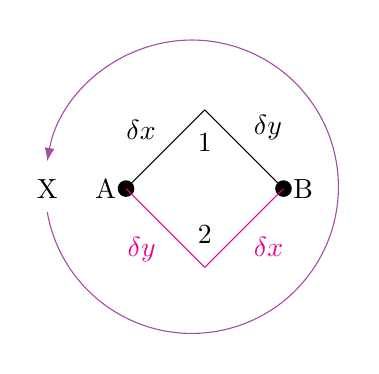
\begin{tikzpicture}
        \fill (0,0) circle (3pt) node[anchor=east] {A};
        \fill (2,0) circle (3pt) node[anchor=west] {B};
        \fill[white] (-1,0) circle (3pt) node[black] {X};
        \draw[-Latex,violet!70!white] (-1,-0.3) arc (-170:170:53pt);
        \draw (0,0) -- (1,1) node[anchor=south east,midway] {$\delta x$} node[anchor=north,yshift=-5pt] {1};
        \draw (1,1) -- (2,0) node[anchor=south west,midway] {$\delta y$};
        \draw[magenta] (0,0) -- (1,-1) node[anchor=north east,midway] {$\delta y$} node[anchor=south,black,yshift=5pt] {2};
        \draw[magenta] (1,-1) -- (2,0) node[anchor=north west,midway] {$\delta x$};
    \end{tikzpicture}
\end{wrapfigure}
If we take two different paths from $A\to B$ in two moves, each to make a loop starting with tensor $\lambda^a$, what is its value at $B$ after travelling the path?
If we denote which path we are considering by $^i$, $i\in\{1,2\}$, then let's start by considering path 1:
\begin{align}
    \lambda^a(B^1) &= \lambda^a(A) + \tensor{\lambda}{^a_{;b}}\delta x^b + \tensor{\lambda}{^a_{;c}}\delta y^c + \tensor{\lambda}{^a_{;b;c}}\delta x^b\delta y^c.
\end{align}
Now if we do path 2:
\begin{align}
    \lambda^a(B^2) &= \lambda^a(A) + \tensor{\lambda}{^a_{;c}}\delta y^c + \tensor{\lambda}{^a_{;b}}\delta x^b + \tensor{\lambda}{^a_{;c;b}}\delta y^c\delta x^b.
\end{align}
For paths 1 and 2, we could get the same answer in flat space as
\begin{align}
    \tensor{\lambda}{^a_{;b;c}}\delta x^b\delta y^c = \tensor{\lambda}{^a_{;c;b}}\delta y^c\delta^b,
\end{align}
but this is not the case in curved space:
\begin{align}
    \begin{split}
        \Delta\lambda^a = \lambda^a(B^2)-\lambda^a(B^1) &= \left(\tensor{\lambda}{^a_{;c;b}}-\tensor{\lambda}{^a_{;b;c}}\right)\delta x^b\delta y^c \\
                                                        &= \tensor{R}{^a_{dbc}}\lambda^a\cdot\text{ area of loop}
    \end{split}
\end{align}
So $\tensor{R}{^a_{dbc}}$ tells us how much a vector swings as we go around a loop. 
The key thing about curvature is that neighbouring geodesics get further apart (or closer together) at a rate depending on the local curvature.
In flat space under no forces, the geodesics are straight lines. 
The distance between two geodesics then increases/decreases linearly as a function of the path length along the geodesic, i.e. \emph{if they start parallel, they stay parallel.}
In curved space, the geodesics do not separate linearly, i.e. the second derivative will not be zero, and this gives us a way to quantify the curvature of spacetime. 
From starting parallel, paths could:
\begin{figure}[H]
    \centering
    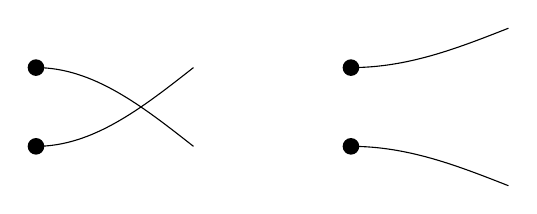
\begin{tikzpicture}
        \fill (0,0) circle (3pt);
        \fill (0,1) circle (3pt);
        \draw (0,0) cos (2,1);
        \draw (0,1) cos (2,0);

        \fill (4,0) circle (3pt);
        \fill (4,1) circle (3pt);
        \draw (4,0) cos (6,-0.5);
        \draw (4,1) cos (6,1.5);
    \end{tikzpicture}
\end{figure}
Consider two geodesics $\gamma$ and $\gamma^a$ with coordinates $x^a(s)$ and $\tilde{x}^a(s)$, and a separation $\zeta^a=\tilde{x}^a - x^a$.
\begin{figure}[H]
    \centering
    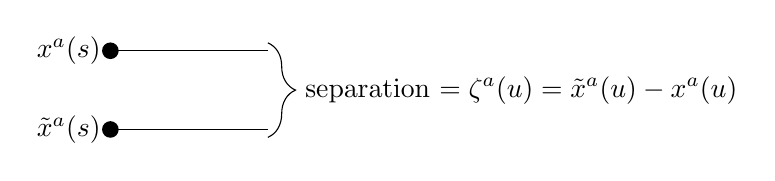
\begin{tikzpicture}
        \fill (0,0) circle (3pt) node[anchor=east] {$\tilde{x}^a(s)$};
        \fill (0,1) circle (3pt) node[anchor=east] {$x^a(s)$};
        \draw (0,0) -- (2,0);
        \draw (0,1) -- (2,1);
        \draw[decorate,decoration={brace,amplitude=10pt,mirror}] (2,-0.1) -- (2,1.1) node[anchor=west,midway,xshift=10pt] {separation $= \zeta^a(u) = \tilde{x}^a(u) - x^a(u)$};
    \end{tikzpicture}
\end{figure}
These are geodesics, so we can use the \emph{geodesic equation:}
\begin{align}
    \frac{d^2x^a}{ds^2} &+ \tensor{\Gamma}{^a_{bc}}\frac{dx^b}{ds} \frac{dx^c}{ds} = 0, & \frac{d^2\tilde{x}^a}{ds^2} &+ \tensor{\tilde{\Gamma}}{^a_{bc}}\frac{d\tilde{x}^b}{ds}\frac{d\tilde{x}^c}{ds} = 0.
\end{align}
We also have $\tilde{x}^a=\zeta^a + x^a$ and $\tilde{x}^c = \zeta^c x^c$, yielding
\begin{align}
    \tensor{\tilde{\Gamma}}{^d_{bc}} &= \tensor{\Gamma}{^a_{bc}}+\frac{\p\tensor{\Gamma}{^a_{bc}}}{\p x^d}(\tilde{x}^d-x^d) = \tensor{\Gamma}{^a_{bc}} + \frac{\p\tensor{\Gamma}{^a_{bc}}}{\p x^d}\zeta^d,
\end{align}
using our separation definition. 
Subtracting the geodesics gives
\begin{align}
    \frac{d^2\tilde{x}^a}{ds^2} + \tensor{\tilde{\Gamma}}{^a_{bc}}\frac{d\tilde{x}^b}{ds}\frac{d\tilde{x}^c}{ds} - \frac{d^2x^a}{ds^2} - \tensor{\Gamma}{^a_{bc}}\frac{dx^b}{ds}\frac{dx^c}{ds} &= 0, \\
    \frac{d^2(x^a+\zeta^a)}{ds^2} + \left(\tensor{\Gamma}{^a_{bc}} + \frac{\p\tensor{\Gamma}{^a_{bc}}}{\p x^d}\zeta^d\right)\frac{d(x^b+\zeta^b)}{ds}\frac{d(x^c+\zeta^c)}{ds} - \frac{d^2x^a}{ds^2} - \tensor{\Gamma}{^a_{bc}}\frac{dx^b}{ds}\frac{dx^c}{ds} &= 0,
\end{align}
and letting the dot denote the derivative with respect to the path length, and keep only the first order terms, i.e. ignore anything with $\dot{\zeta}\dot{\zeta}$, yields
\begin{align}
    \ddot{\zeta}^a &+ \tensor{\Gamma}{^a_{bc}}\dot{x}^b\dot{\zeta}^c + \tensor{\Gamma}{^a_{bc}}\dot{\zeta}^b\dot{x}^c + \frac{\p\tensor{\Gamma}{^a_{bc}}}{\p x^d} \zeta^d\dot{x}^b\dot{x}^c = 0.
\end{align}
We have this term $\ddot{\zeta}^a$, but we are looking for a tensor equation, and we would get something with this term that transformed as a tensor if we had $\frac{D^2\zeta}{ds^2}$ instead:
\begin{align}
    \begin{split}
        \frac{D^2\zeta^a}{ds^2} &= \frac{D}{ds}\left(\dot{\zeta}^a + \tensor{\Gamma}{^a_{bc}}\zeta^b\dot{x}^c\right) = \frac{D}{ds}\dot{\zeta}^a + \frac{D}{ds}\left(\tensor{\Gamma}{^a_{bc}}\zeta^b\dot{x}^c\right) \\
                                &= \ddot{\zeta}^a + \tensor{\Gamma}{^a_{bc}}\zeta^b\dot{x}^c + \frac{d}{ds}\left(\tensor{\Gamma}{^a_{bc}}\zeta^b\dot{x}^c\right)+\tensor{\Gamma}{^a_{ef}}\left(\tensor{\Gamma}{^e_{bc}}\zeta^b\dot{x}^c\right)\dot{x}^f.
    \end{split}
\end{align}
Let's substitute our expression involving $\frac{d^2\zeta^a}{ds^2}$ (which is not a tensor) into our expression for $\frac{D^2\zeta^a}{ds^2}$ (which is a tensor).
Looking at the term $\frac{d}{ds}(\tensor{\Gamma}{^a_{bc}}\zeta^b\dot{x}^c)$:
\begin{align}
    \frac{d}{ds}\left(\tensor{\Gamma}{^a_{bc}}\zeta^b\dot{x}^c\right) &= \tensor{\Gamma}{^a_{be}}\zeta^b\ddot{x}^e + \zeta^b\dot{x}^c\left(\frac{\p\tensor{\Gamma}{^a_{bc}}}{\p x^d}\dot{x}^d\right) + \tensor{\Gamma}{^a_{bc}}\dot{\zeta}^b\dot{x}^c.
\end{align}
The first of these can be rewritten because te path is a geodesic, so
\begin{align}
    \ddot{x}^e &= -\tensor{\Gamma}{^e_{cd}}\dot{x}^c\dot{x}^d.
\end{align}
The third term (with $\dot{\zeta}^b$) is just the same as the $\dot{\zeta}^c$ terms in our expression for $\ddot{\zeta}^a$.
If we work through the algebra, combining Eqs (9.19) and (9.20) and do lots of relabelling, we get
\begin{align}
    \frac{D^2\zeta^a}{ds^2} + \left(\tensor{\Gamma}{^a_{be}}\tensor{\Gamma}{^e_{cd}} - \tensor{\Gamma}{^a_{ce}}\tensor{\Gamma}{^e_{bd}} + \frac{\p\tensor{\Gamma}{^a_{cd}}}{\p x^d} - \frac{\p\tensor{\Gamma}{^a_{bd}}}{\p x^c}\right)\zeta^b\dot{x}^c\dot{x}^d &= 0.
\end{align}
So here we have something which should equal zero if the space is flat, and not zero if the space is curved, but this is just the \emph{Riemann curvature tensor!}
\begin{align}
    \frac{D^2\zeta^a}{ds^2} &+ \tensor{R}{^a_{dbc}}\zeta^b\dot{x}^c\dot{x}^d = 0, \\
    \tensor{R}{^a_{dbc}} &= \left(\tensor{\Gamma}{^a_{be}}\tensor{\Gamma}{^e_{cd}} - \tensor{\Gamma}{^a_{ce}}\tensor{\Gamma}{^e_{bd}} + \p_b\tensor{\Gamma}{^a_{cd}} - \p_c\tensor{\Gamma}{^a_{bd}}\right).
\end{align}
This tensor equation does not care about coordinate systems. 
Flat space has all components of $\tensor{R}{^a_{bcd}}=0$ irrespective of whether you are working in spherical polar coordinates or Cartesian coordinates, and if all components are zero then $\frac{D^2\zeta^a}{ds^2}=0,\zeta^a=Au+B$, so geodesics in flat space separate linearly (or remain parallel if $A=0$).
Geodesics in curved space do not. 

\chapter{Symmetries of the Riemann Tensor and Implications}
\emph{Things are about to get a little more physics!} - Richard Bower. 
\begin{itemize}
    \item Symmetry of the Riemann tensor,
        \begin{align}
            \tensor{R}{^a_{dbc}} &= \tensor{\Gamma}{^a_{bc}}\tensor{\Gamma}{^e_{cd}} - \tensor{\Gamma}{^a_{ce}}\tensor{\Gamma}{^e_{bd}} + \p_b\tensor{\Gamma}{^a_{cd}}-\p_c\tensor{\Gamma}{^a_{bd}}.
        \end{align}
    \item We will look towards Einstein's equations by combining our knowledge of movement in curved space with gravity.
    \item We will do this through the stress-energy tensor, $T^{\mu\nu}$. (Not as simple as it could be, R has four indices, this has two, but we'll get to that.)
    \item This will lead towards to conservation laws in GR.
\end{itemize}
At the end of last lecture, we considered divergent lines with a spatially-dependent separation $\zeta$:
\begin{align}
    \ddot{x}^a + \tensor{\Gamma}{^a_{bc}}\dot{x}^b\dot{x}^c &= 0 \\
    \ddot{\tilde{x}}^a + \tensor{\tilde{\Gamma}}{^a_{bc}}\dot{x}^b\dot{x}^c &= 0 \\
    \ddot{\zeta} + \tensor{\Gamma}{^a_{bc}}\dot{x}^b\dot{\zeta}^c + \tensor{\Gamma}{^a_{bc}}\dot{\zeta}^b\dot{x}^c + \frac{\p\tensor{\Gamma}{^a_{bc}}}{\p x^d}\zeta^d\dot{x}^b\dot{x}^c &= 0.
\end{align}
We want to find the Tensor equation from this!
\begin{align}
    \frac{D^2\zeta^a}{ds^2} &= \ddot{\zeta}^a + \tensor{\Gamma}{^a_{bc}}\dot{\zeta}^b\dot{x}^c + \frac{d}{ds}\left(\tensor{\Gamma}{^a_{bc}}\zeta^b\dot{x}^c\right) + \tensor{\Gamma}{^a_{ef}}\left(\tensor{\Gamma}{^a_{bc}}\zeta^b\dot{x}^c\right)\dot{x}^f.\\
    \frac{d}{ds}\left(\tensor{\Gamma}{^a_{bc}}\zeta^b\dot{x}^c\right) &= \tensor{\Gamma}{^a_{be}}\zeta^b\ddot{x}^e + \tensor{\Gamma}{^a_{bc}}\dot{\zeta}^b\dot{x}^c + \zeta^b\dot{x}^c\left(\frac{\p\tensor{\Gamma}{^a_{bc}}}{\p x^d}\dot{x}^d\right).
\end{align}
So we expanded out the derivative to get rid of something we didn't want, and now combine for the final result (as well as using the definition of a geodesic path, $\ddot{x}^e=-\tensor{\Gamma}{^e_{cd}}\dot{x}^c\dot{x}^d$, in Eq. (10.5)):
\begin{align}
    \frac{D^s\zeta^a}{ds^2} &+ \left(\tensor{\Gamma}{^a_{be}}\tensor{\Gamma}{^e_{cd}}-\tensor{\Gamma}{^a_{ce}}\tensor{\Gamma}{^e_{bd}}+\p_b\tensor{\Gamma}{^a_{cd}}-\p_c\tensor{\Gamma}{^a_{bd}}\right)\zeta^b\dot{x}^c\dot{x}^d = 0.
\end{align}
This looks very confused as it is, but we can simplify by now defining the Riemann tensor:
\begin{align}
    \frac{D^2\zeta}{ds^2} &+ \tensor{R}{^a_{dbc}}\zeta^b\dot{x}^c\dot{x}^d = 0,\\
    \tensor{R}{^a_{dbc}} &= \tensor{\Gamma}{^a_{bc}}\tensor{\Gamma}{^e_{cd}} - \tensor{\Gamma}{^a_{ce}}\tensor{\Gamma}{^e_{bd}} + \p_b\tensor{\Gamma}{^a_{cd}}-\p_c\tensor{\Gamma}{^a_{bd}}.
\end{align}
From this definition, we can quickly infer the symmetry relation
\begin{align}
    \tensor{R}{^a_{dcb}} &= -\tensor{R}{^a_{dbc}}.
\end{align}
We can write the Riemann tensor out in full, but it is very big and tedious. 
In 4D spacetime, the Riemann tensor contains $4\times4\times4\times4 = 256$ numbers.
This isn't very fun unless you are a computer, says Richard.
However, the \emph{symmetry properties} of the Riemann tensor mean that it only has 20 algebraically-independent components. 
How do we demonstrate this though?
We can use mathematical tricks for tensors, whereby if we prove something in one coordinate system, it must be true in all coordinate systems.

\section{Local Geodesic Coordinates}
We can always define locally-geodesic coordinates: those in which the metric tensor is given by $\eta_{\alpha\beta}$ and the Christoffel symbols are zero, but their derivatives are \unl{not.}
We cannot transform gravity away in a global sense. 
In what follows, we are looking the components of the curvature tensor in the \emph{local geodesic frame.}
Local geodesic coordinates describe a flat space at a local point in curved space.
We know, therefore, that we can write the metric at this point as
\begin{align}
    g_{\alpha\beta} &= \begin{pmatrix} 1 & 0 & 0 & 0 \\ 0 & -1 & 0 & 0 \\ 0 & 0 & -1 & 0 \\ 0 & 0 & 0 & -1 \end{pmatrix},
\end{align}
which is known as the \textbf{Minkowski metric} for flat space.
This is familiar from special relativity, where it represents the usual Minkowski product,
\begin{align}
    ds^2 &= c^2\,d\tau^2 = c\,dt^2 - dx^2 - dy^2 - dz^2.
\end{align}
So the Christoffel symbol at this local point is
\begin{align}
    \tensor{\Gamma}{^\alpha_{\beta\gamma}} &= 0,
\end{align}
where we have only chosen a point to set this locally to zero.
However, the derivatives will not be zero, as if we move away from this local point, space will become curved again:
\begin{align}
    \frac{\p\tensor{\Gamma}{^\alpha_{\beta\gamma}}}{\p x^\delta} &\neq 0.
\end{align}
Now this will allow us to simplify the Riemann tensor from its definition in Eq. (10.9), where it can now be written as
\begin{align}
    \tensor{R}{^a_{dbc}} &= \p_b\tensor{\Gamma}{^a_{cd}} - \p_c\tensor{\Gamma}{^a_{bd}}.
\end{align}
What about the symmetry relations of this simplified Riemann tensor?
\begin{align}
    \tensor{R}{^a_{cdb}} &= \p_d\tensor{\Gamma}{^a_{bc}} - \p_b\tensor{\Gamma}{^a_{dc}}, \\
    \tensor{R}{^a_{bcd}} &= \p_c\tensor{\Gamma}{^a_{db}} - \p_d\tensor{\Gamma}{^a_{cb}}.
\end{align}
What about the sum of these three tensors?
Due to the symmetry of the Christoffel symbols' lower indices, we can see that there will be lots of cancellations in this sum, leading to
\begin{align}
    \tensor{R}{^a_{dbc}} + \tensor{R}{^a_{cdb}} + \tensor{R}{^a_{bcd}} &= 0,
\end{align}
which is known as the cyclic relation of the Riemann tensor.
This is a \emph{tensor equation} so even though we derive it in the local frame, it must be true in all frames. 
The Riemann tensor can also be written in its covariant form:
\begin{align}
    \tensor{R}{_{abcd}} &= g_{ae}\tensor{R}{^e_{bcd}} = g_{ac}\left[\p_c\tensor{\Gamma}{^e_{db}} - \p_d\tensor{\Gamma}{^e_{cb}}\right].
\end{align}
As we can take $g_{ae}$ inside the partial derivatives, the covariant derivative reduces to the partial derivative, giving
\begin{align}
    R_{abcd} &= \p_c\Gamma_{adb}-\p_d\Gamma_{acd}.
\end{align}
These Christoffel symbols can be written in terms of the derivatives of the metric where we had:
\begin{align}
    \Gamma_{abc} &= g_{af}\tensor{\Gamma}{^f_{bc}} = \frac12 g_{af}g^{fe}\left(\p_bg_{ec} - \p_eg_{cb} + \p_cg_{be}\right),\\
    \begin{split}
        R_{abcd} &= \frac12\p_c\left[\p_dg_{ab} + \p_bg_{da} - \p_ag_{db}\right] - \frac12\p_d\left[\p_cg_{ab} + \p_bg_{ca} - \p_ag_{cb}\right] \\
                 &= \frac12\left(\p_a\p_dg_{bc} - \p_b\p_dg_{ac} + \p_b\p_cg_{ad} - \p_a\p_cg_{bd}\right),
    \end{split}
\end{align}
where we use the fact that $g_{ab}=g_{ba} \implies \p_d\p_dg_{ab} = \p_c\p_dg_{ab}$.
From these symmetry relations, we see that:
\begin{align}
    R_{abcd} &= -R_{bacd}, & R_{abcd} &= -R_{abdc}, & R_{abcd} &= R_{cdab}.
\end{align}
These are tensor equations, so must be true in all frames. 
This shows us that there are a lot of $R_{abcd}=0$, as if we have a repeated index in the first two places, and the only way that a number can be equal to its own negative if it is equal and similarly for a repeated index on the last two places, i.e.
\begin{align}
    \begin{split}
        R_{aacd} = -R_{aacd} &\implies R_{aacd} = 0, \\
        R_{abcc} = -R_{abcc} &\implies R_{abcc} = 0.
    \end{split}
\end{align}
This allows us to neglect many of the 256 numbers as they will be zero, reducing the total of free elements of the Riemann tensor to 20.

\section{Towards Einstein's Equations}
The curvature of space is related to tidal force, i.e. to the $\frac{M}{R^3}$ which is the density of mass. 
We want some tensor equation (valid in any frame) such that curvature is equivalent to gravity, so an equation (tensor) linking the Riemann curvature tensor and mass density.
Einstein said that mass and energy are equivalent, so all forms of energy (not just mass) should gravitate.
In Newtonian gravity, two particles are initially at rest at the same radial distance $x$ with a separation $y$ ($y\ll x$) from a star of mass $M$.
They are accelerated radially by the gravitational force, $\propto \frac{GM}{r^2}$.
\begin{figure}[H]
    \centering
    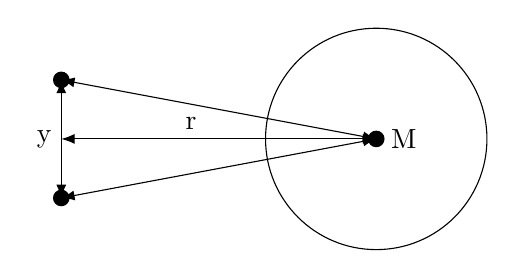
\begin{tikzpicture}
        \fill (0,0) circle (3pt);
        \fill (0,1.5) circle (3pt);
        \fill (4,0.75) circle (3pt);
        \draw (4,0.75) circle (40pt) node[xshift=10pt] {M};
        \draw[Latex-Latex] (0,0) -- (0,1.5) node[anchor=east,midway] {y};
        \draw[Latex-Latex] (0,0.75) -- (4,0.75) node[anchor=south,midway,xshift=-10pt] {r};
        \draw[Latex-Latex] (0,0) -- (4,0.75);
        \draw[Latex-Latex] (0,1.5) -- (4,0.75);
    \end{tikzpicture}
\end{figure}
Let's consider Eq. (10.4) for low speeds, i.e. non-relativistic.
\begin{align}
    \zeta^\alpha = \begin{pmatrix} 0, & 0, & y, & 0 \end{pmatrix},
\end{align}
i.e. we have a simple separation in the y-direction between the two geodesic paths.
We would then get something like
\begin{align}
    \frac{D^2y}{ds^2} &= -\tensor{R}{^2_{020}}yc^2,
\end{align}
where we only consider the indices relating to $y$ and time.
This should look somewhat familiar.
What would we have written for this in Newtonian physics?
Since they are in free-fall, they are travelling on geodesics and these are getting closer together as the particles fall towards the star. 
Resolving the radial force on one of the stars into a force along the same direction as the other radial force, and one perpendicular to it, then there is a force towards the other particle of
\begin{align}
    \frac{d^2y}{dt^2} &= -\frac{GM}{r^2}\cdot\frac{y}{r},
\end{align}
and the distance apart is $\approx y$.
This shows an acceleration term between the two particles. 
Important note: the massive object is the Sun or a molecular cloud or something, according to Richard.
\textbf{A black hole wouldn't be happy, you wouldn't be able to tell.}\\
Converting to \emph{path length} and using $ds=c\,dt$:
\begin{align}
    \frac{d^2y}{ds^2}\left(\frac{ds}{dt}\right)^2 = c^2\frac{d^2y}{ds^2} &= -\frac{GM}{r^3}y.
\end{align}
Compare this with the curvature tensor:
\begin{align}
    \frac{D^2\zeta^a}{ds^2} &= -\tensor{R}{^a_{cbd}}\zeta^b\dot{x}^c\dot{x}^d.
\end{align}
The biggest term again is for $c=d=0$, so
\begin{align}
    \frac{D^2\zeta^a}{ds^2} &= -\tensor{R}{^a_{0b0}}\zeta^bc^2.
\end{align}
$\zeta^a$ is the separation as in Eq. (10.25), as both particles have the same $t,x,$ and $z$ then there is only separation in $y$ so this becomes Eq. (10.26) and then we can show the equivalence of curved space and Newtonian force as
\begin{align}
    -\frac{GM}{r^3} &= -\tensor{R}{^2_{020}}.
\end{align}
We see that the tidal forces which we would associate with gravity can be made simply from curved space. 
We can see that this Newtonian expression is the \textbf{Energy Density of Space}, if mass and energy can be equivalent.
This is what lead Einstein to his famous equations.
The curvature tensor in some sense tells us about \emph{tidal forces} - how gravity changes force point to point. 
In flat space, all
\begin{align}
    \tensor{R}{^a_{cbd}} = 0 \implies \frac{D^2\zeta^a}{ds^2} = 0,
\end{align}
and geodesics separate as $\zeta^a=Au+B$, i.e. in flat space, geodesics either maintain a constant separation (parallel lines) or separate/approach linearly. 
With no gravity, things continue in straight lines at constant velocity. 

\section{The Stress-Energy Tensor}
In \emph{special relativity}, if you accelerate a particle, giving it more and more energy, then as you approach $c$ then the mass increases rather than the velocity. 
This is arbitrary unless all forms of energy gravitate as then as we add energy, we increase the inertial (e.g. gravitational) mass. 
In special relativity, we generally dealth with individual particles, where
\begin{align}
    E &= \gamma m_0c^2,
\end{align}
was the particle energy, relating the mass and energy of objects.
Recall again from special relativity the four-velocity of a system:
\begin{align}
    u^\alpha &= \frac{dx^\alpha}{dt} = \gamma\begin{pmatrix} c, & -\frac{dx^i}{dt}\end{pmatrix}.
\end{align}
There is also the four-momentum of the system:
\begin{align}
    p^\alpha &= m_0u^\alpha = \gamma m_0\begin{pmatrix} c, & -\frac{dx^i}{dt} \end{pmatrix}.
\end{align}
A stationary particle has $p^\mu = m_0(c,0,0,0)$, and while moving has
\begin{align}
    p^\alpha = \gamma m_0\begin{pmatrix} c, & \frac{dx^1}{dt}, & \frac{dx^2}{dt}, & \frac{dx^3}{dt} \end{pmatrix}.
\end{align}
We  want to generalise these to look at density, but density is a frame-dependent quantity, which is a problem. 
The total number of particles in a given volume must be invariant, but the volume changes by length contraction along the direction of motion, so if we have a number density, $n_0$, in the rest frame for the number of particles ``in a box" or in the universe or whatever you're considering, then $n_0\gamma$ is the number density as measured in a moving frame. 
If we are now moving, there is a flux of particles across the surfaces, i.e. we take two separate concepts (density and flux) and make them into a single 4-vector, the number-flux 4-vector:
\begin{align}
    N^\mu &= n_0u^\mu.
\end{align}
This is a 4-vector as it transforms in the right way for a contravariant tensor.
In the rest frame, $N^\mu = n_0\frac{dx^\mu}{d\tau}$; in a moving frame, then
\begin{align}
    N^{\nu'} &= n\frac{dx^{\nu'}}{d\tau} = n_0\frac{dx^{\nu'}}{dx^\mu}\frac{dx^\mu}{d\tau} = \frac{dx^{\nu'}}{dx^\mu}N^\mu.
\end{align}
Alernatively, since we know $u^\mu$ is a 4-vector and so since $N^\mu$ is related to it only by invariant quantities (not frame density) then this must also be a 4-vector. 

Now we want \emph{energy density.}
In the rest frame, if particles have no velocity relative to each other, then the energy density is just $m_0c^2n_0 = \rho_0c^2$, where $\rho_0$ is the mass density in the rest frame.
If we go to another frame, we have to transform the energy and the density, so it tramsforms by two factors of $\gamma$, so this needs to be a second-order contravariant tensor. 
So now we introduce the \textbf{Stress-Energy Tensor} as an expression for the energy-momentum density:
\begin{align}
    T^{\mu\nu} &= N^\mu p^\nu = n_0u^\mu m_0u^\nu = \rho_0 u^\mu u^\nu.
\end{align}
In the rest frame, this would have only one component, $T^{00}=n_0cm_00=\rho_0c^2$, as we had before in the rest frame.

\chapter{Conservation Laws and Einstein's Equations}
The results for the stress-energy tensor from the last lecture only works if we are dealing with \emph{dust}, i.e. something where the particles have no internal motions, and no stresses or heat conduction or anything complicated.
However in general a gas \unl{has} internal motion - particles are moving with respect to each other so there is no rest frame as such for each particle, only a rest frame for the gas as a whole. 
In the rest frame, 
\begin{align}
    u = (c,0,0,0) \implies T^{00} = \rho_0c^2.
\end{align}
We get relevant fluxes setting one 0 to non-zero (where $i\in\{1,2,3\}$ for spatial direction):
\begin{itemize}
    \item $T^{0i} =$ energy flux through a surface $i$;
    \item $T^{ii} =$ momentum in a particular direction $i$;
    \item $T^{ii} =$ momentum flux through a surface $i$.
\end{itemize}
We can define a more general $T^{\mu\nu}$ by considering what happens for a \emph{perfect fluid} - a gas with both rest mass and internal motions. 
We have to take into account \emph{pressure}, not just energy.
From special relativity, we know that the energy of this in the rest frame is
\begin{align}
    3p = 3n_0k_BT,
\end{align}
so the total energy density in the rest frame is $\rho_0c^2 + 3n_0k_BT$, so
\begin{align}
    T^{\mu\nu} = \begin{pmatrix} \rho_0c^2 & 0 & 0 & 0 \\ 0 & -p & 0 & 0 \\ 0 & 0 & -p & 0 \\ 0 & 0 & 0 & -p \end{pmatrix},
\end{align}
where $\rho_0c^2$ is the rest mass energy of the gas and $-p$ are the contributions from the pressures of the gas on the walls.
In general, we can then write
\begin{align}
    T^{\mu\nu} = \left(\rho_0+\frac{p}{c^2}\right)u^\mu u^\nu - pg^{\mu\nu}.
\end{align}
In flat space, our metric for this is the \emph{Minkowski metric tensor}:
\begin{align}
    \begin{split}
        g^{\mu\nu} &= \text{diag}(1,-1,-1,-1), \\
        ds^2 &= g^{\alpha\beta}dx^\alpha dx^\beta = c^2dt^2 - dx^2 - dy^2 - dz^2.
    \end{split}
\end{align}
We see the result is a tensor as it is made out of things that are either \emph{invariant} (scalars) or \emph{tensors.}
In the rest frame, it has components
\begin{align}
    T^{00} &= \left(\rho_0+\frac{p}{c^2}\right)c^2-p = \rho_0c^2, & T^{ii} &= -p\times(-1) = p,
\end{align}
so it has the right form in the rest frame. 
Since we have the metric, we can use this in general relativity. 
It is a \emph{symmetric tensor}, $T^{\mu\nu}=T^{\nu\mu}$, as $g^{\mu\nu}$ is symmetric and $u^\mu u^\nu = u^\nu u^mu$.
The pressure contributes to the energy density, and energy density curves space through increasing $T^{\mu\nu}$.
So for the interior of a star, as the fuel runs out then the star contracts and gravity gets stronger. 
We require a larger pressure to hold the star up, but this pressure adds to the total energy density, so increases gravity, so more pressure is needed...etc; pressure outweights force from gas. 
This process will of course eventually lead to the formation of \textbf{Black Holes.}

\section{Conservation Laws}
The stress-energy tensor for a perfect fluid in special relativity which we defined above is a very compact way to count up all the contributions to the energy density and it is a tensor so it works in all (inertial) frames. 
It can be made more general as $T^{\mu\nu}$ is defined as the flow of momentum associated with $x^\mu$ across the $x^\nu$ surface. 
$T^{ij}\; (i\neq j)$ is the \emph{shear stress} so these are zero for a perfect fluid.
Pressure forces are perpendicular to the surface (no shear stresses).
It also embodies information - energy is conserved. 

Considering the rate of change of energy in a volume:
\begin{figure}[H]
    \centering
    \begin{tikzpicture}
        \draw (0,0) -- (3,0) node[anchor=north,midway] {$l$} -- (3,3) -- (0,3) -- cycle;
        \draw (3,0) -- (4,0.5) -- (4,3.5) -- (1,3.5) -- (0,3);
        \draw (4,3.5) -- (3,3);
        \draw[-{Latex[length=3mm,width=2.5mm]}] (-0.7,-0.1) -- (1.5,1.5);
        \draw[-{Latex[length=3mm,width=2.5mm]}] (4,3.3) -- (4.8,3.9);
    \end{tikzpicture}
    \vspace{-40pt}
\end{figure}
\begin{align}
    \text{Rate of change } &= \text{ Energy flux in } - \text{ Energy flux out},\\
    \begin{split}
        l^3\frac{\p T^{00}(x)}{\p t} &\approx l^2cT^{01}(x) - l^2cT^{01}(x+l) = l^2c\left(T^{01}(x) - T^{01}(x+l)\right) \\
                                     &= -l^2c\left(\frac{\p T^{01}}{\p x}\right)l = -l^3c\frac{\p T^{01}}{\p x}.
    \end{split}
\end{align}
This is in 1D so we need similar contributions from the other two pairs of faces so we have:
\begin{align}
    l^3c\frac{\p T^{00}(x)}{c\p t} &= -l^3c\frac{\p T^{01}}{\p x} - l^3c\frac{\p T^{02}}{\p y} - l^3c\frac{\p T^{03}}{\p z} = -l^3c\frac{\p T^{0i}}{\p x^i}, \\
    \frac{\p T^{00}}{c\p t} &= -\frac{\p T^{0i}}{\p x^i} \implies \frac{\p T^{00}}{c\p t} + \frac{\p T^{0i}}{\p x^i} = 0.
\end{align}
Remebering that $ct$ is just the 0th component, we can see that a total summation will make this look very simple:
\begin{align}
    \frac{\p T^{0\alpha}}{\p x^\alpha} &= 0.
\end{align}
In other words, $\p_\alpha T^{i\alpha} = 0$, which contains conservation of momentum so both momentum and energy are embodied in $\p_\alpha T^{\alpha\beta} = 0$.
We can also write this using the covariant derivative:
\begin{align}
    \tensor{T}{^{0\alpha}_{;d}} &= 0, & \tensor{T}{^{i\alpha}_{;d}} &= 0, & \tensor{T}{^{\alpha\beta}_{;d}} &= 0.
\end{align}
Then, remembering the symmetry of the tensor:
\begin{align}
    T^{\alpha\beta} &= T^{\beta\alpha}, & \tensor{T}{^{\alpha\beta}_{;\alpha}} &= 0.
\end{align}
Any physical law which can be expressed in tensor notation in special relativity has exactly the same form in a locally-inertial frame of a curved spacetime, i.e. general relativity. 
Locally-inertial frames are equivalent to saying we choose to look at a small piece of spacetime, where we can approximate any curved space to a locally-flat space. 
In this choice of coordinates, all the \emph{Christoffel symbols} are zero so standard differentiation and covariant differentiation are the same. 
Outside of this, curvature becomes apparent. 
To make tensor equations work in any general frame, we need to swap standard differentiation with covariant differentiation, e.g.
\begin{align}
    \tensor{T}{^{\alpha\beta}_{;\alpha}} &= 0.
\end{align}

\section{Einstein's Equations}
We want a tensor equation which has \emph{curvature-energy density.}
The stress-energy tensor is second-order, and has a covariant derivative of zero as this embodies the conservation laws for energy and momentum. 
So we are looking for a way to denote curvature which is also a second-order symmetric tensor with covariant derivative of zero. 
The \emph{Riemann curvature tensor} completely embodies all the information about the curvature of space, and is a \emph{fourth-order tensor.}
Connecting:
\begin{align}
    T^{\alpha\beta} \iff \tensor{R}{^\alpha_{\beta\gamma\delta}},
\end{align}
where we have 2 indices, then 4.
There is no way that a second-order tensor can be equal to a fourth-order one. 
We need to \emph{contract} the Riemann curvature tensor, preferably without losing any information about the spatial curvature. 
We know from index symmetries that
\begin{align}
    R_{abcd} &= -R_{bacd}, & R_{abcd} &= -R_{abdc}, & R_{abcd} &= R_{cdab},
\end{align}
so we can get fewer independent components.
We introduce the \textbf{Ricci tensor} to solve this issue. 
To contract $\tensor{R}{^a_{bcd}}$, we could sum over one of the covariant indices with the contravariant one. 
Which covariant index? 
In principle, $\tensor{R}{^a_{acd}}\neq\tensor{R}{^a_{bad}}\neq\tensor{R}{^a_{bca}}$.
If we contract over the first index, i.e. $\tensor{R}{^a_{acd}}$, then we can see that
\begin{align}
    \tensor{R}{^a_{acd}} &= g^{ae}R_{eacd} = -g^{ae}R_{aecd} = -g^{ea}R_{aecd} = -\tensor{R}{^e_{ecd}} = -\tensor{R}{^a_{acd}}.
\end{align}
The only way this can be true in general is if $\tensor{R}{^a_{acd}}=0$, so this is not a useful index to contract over. 
We can contract over index 3 or 4.
Since 
\begin{align}
    R_{abcd} &= -R_{abdc}, & \tensor{R}{^a_{bad}} &= \tensor{R}{^a_{bda}} = R_{bc},
\end{align}
where $R_{bc}$ is the \textbf{Ricci tensor.}
We can multiply by the metric twice to change indices, i.e. contravariant. 
The Ricci tensor is a second-order tensor about the source of gravity (energy density).
Let's try
\begin{align}
    R^{\mu\nu} &= \kappa T^{\mu\nu}
\end{align}
as the equation we are after.
The \emph{Ricci tensor} is also \emph{symmetric}, i.e. $R_{bc} = R_{cb}$.
Using local geodesic coordinates, all Christoffel symbols equal zero locally, but derivatives are non-zero.
This makes the covariant derivative easier:
\begin{align}
    \tensor{R}{^a_{bcd}} &= \p_c\tensor{\Gamma}{^a_{db}} - \p_d\tensor{\Gamma}{^a_{cb}}, \\
    \begin{split}
        \tensor{R}{^a_{bcd;e}} &= \p_e\left(\p_c\tensor{\Gamma}{^a_{db}} - \p_d\tensor{\Gamma}{^a_{cb}}\right) \\
                               &= \p_e\p_c\tensor{\Gamma}{^a_{db}} - \p_e\p_d\tensor{\Gamma}{^a_{cb}},
    \end{split}
\end{align}
Then, cycling around indices:
\begin{align}
    \tensor{R}{^a_{bde;c}} &= \p_c\p_d\tensor{\Gamma}{^a_{be}} - \p_c\p_e\tensor{\Gamma}{^a_{bd}},\\
    \tensor{R}{^a_{bec;d}} &= \p_d\p_e\tensor{\Gamma}{^a_{bc}} - \p_d\p_c\tensor{\Gamma}{^a_{be}},
\end{align}
where the components here all cancel due to symmetries. 
This then results in
\begin{align}
    \tensor{R}{^a_{bcd;e}} + \tensor{R}{^a_{bde;c}} + \tensor{R}{^a_{bec;d}} = 0.
\end{align}
Again, this is a tensor equation, so it holds in all frames, not just the locally-inertial frame. 
We can use the \emph{Bianchi identity} to get this for the Ricci tensor:
\begin{align}
    \tensor{R}{^a_{bca;e}} + \tensor{R}{^a_{bae;c}} + \tensor{R}{^a_{bec;a}} &= 0,\\
    \tensor{R}{_{bc;e}} - \tensor{R}{_{be;c}} + \tensor{R}{^a_{bec;a}} &= 0.
\end{align}
Note that the last term of this will not simplify.
We can then raise the index $b$ by multiplying by the metric, $g^{fb}$:
\begin{align}
    g^{fb}\tensor{R}{_{bc;e}} - g^{fb}\tensor{R}{_{be;c}} + g^{fb}\tensor{R}{^a_{bec;a}} &= 0 \implies \tensor{R}{^f_{c;e}} - \tensor{R}{^f_{e;c}} + \tensor{R}{^{af}_{ec;a}} = 0.
\end{align}
We also have the curvature index $R=R^a_a$, known as the \textbf{Riemann curvature scalar}, by contracting $e\to f$:
\begin{align}
    \tensor{R}{^f_{c;f}} - \tensor{R}{^f_{f;c}} + \tensor{R}{^{af}_{fc;a}} &= 0 \implies
    \tensor{R}{^f_{c;f}} - \tensor{R}{_{;c}} + \tensor{R}{^{af}_{fc;a}} = 0.
\end{align}
Switching indices in the last term top and bottom so there is no minus sign added yields:
\begin{align}
    \tensor{R}{^f_{c;f}} - \tensor{R}{_{;c}} + \tensor{R}{^{fa}_{cf;a}} &= 0 \implies 
    \tensor{R}{^f_{c;f}} - \tensor{R}{_{;c}} + \tensor{R}{^{a}_{c;a}} = 0,\\
    2\tensor{R}{^a_{c;a}} - \tensor{R}{_{;c}} &= 0 \implies
    \left(\tensor{R}{^a_c} - \frac12R\tensor{\delta}{^a_c}\right)_{;a} = 0.
\end{align}
Multiplying by $g^{bc}$ to raise the index on the bottom and replacing $c$ by $a$:
\begin{align}
    \left(R^{ab} - \frac12g^{ab}R\tensor{\delta}{^a_c}\right)_{;a} &= 0,\\
    \left(R^{ab} - \frac12g^{ab}R\right)_{;a} &= 0.
\end{align}
So the covariant derivative of the Ricci tensor is \unl{not} zero, but the combination of the Ricci tensor and curvature scalar is, i.e. $T^{\alpha\beta}=R^{\alpha\beta}$ is \textbf{wrong.}\\
The combination above does have zero divergence, and is just a function of curvature, so
\begin{align}
    T^{\alpha\beta} &= R^{\alpha\beta} - \frac12g^{\alpha\beta}R.
\end{align}
This describes how energy, pressure, and momentum contribute to the curvature of the universe.

\chapter{}
There can be a scalar relationship for the stress-energy equation described last lecture, i.e.
\begin{align}
    \kappa T^{\alpha\beta} &= R^{\alpha\beta} - \frac12 g^{\alpha\beta}R,
\end{align}
and there could also be an \emph{integration constant,} i.e.
\begin{align}
    \kappa T^{\alpha\beta} &= R^{\alpha\beta} - \frac12g^{\alpha\beta}R + g^{\alpha\beta}\Lambda,
\end{align}
where $\Lambda$ is the \emph{cosmological constant.}
Einstein added this because he wanted a static universe. 
This leads us to the \textbf{Einstein equation,}
\begin{align}
    R^{\mu\nu} - \frac12g^{\mu\nu}R &= \kappa T^{\mu\nu} + g^{\mu\nu}\Lambda,
\end{align}
which finally allows us to equate curvature to gravity. 
For black holes, which will be our primary focus from now, the cosmological constant is not important, so we will set $\Lambda=0$, i.e. strong gravity dominates.

\section{Recasting Einstein's Field Equation}
Neglecting the cosmological constant, starting with Eq (12.1) and multiplying by $g_{\gamma\alpha}$,yields
\begin{align}
    g_{\gamma\alpha}R^{\alpha\beta} - \frac12g_{\gamma\alpha}g^{\alpha\beta}R &= \kappa g_{\gamma\alpha}T^{\alpha\beta}, \\
    \tensor{R}{^\beta_\gamma} - \frac12\tensor{\delta}{^\beta_\gamma}R &= \kappa\tensor{T}{^\beta_\gamma}.
\end{align}
Then, if we contract these sums by setting $\beta=\gamma$, and recall $\tensor{\delta}{^\beta_\beta}=4$, we find
\begin{align}
    \tensor{R}{^\beta_\beta} - \frac12\tensor{\delta}{^\beta_\beta}R &= \kappa\tensor{T}{^\beta_\beta}, \\
    R - 2R &= \kappa T \implies R = -\kappa T.
\end{align}
If we then substitute this definition into our equation, we arrive at an alternative form:
\begin{align}
    \begin{split}
        R^{\alpha\beta} &= \kappa T^{\alpha\beta} + \frac12g^{\alpha\beta}(-\kappa T) \\
        R^{\alpha\beta} &= \kappa\left(T^{\alpha\beta} - \frac12g^{\alpha\beta}T\right),
    \end{split}
\end{align}
which we can compare with 
\begin{align}
    \kappa T^{\alpha\beta} &= \left(R^{\alpha\beta} - \frac12g^{\alpha\beta}R\right).
\end{align}
Since $\alpha,\beta=\{0,1,2,3\}$, $A^{\alpha\beta}$ has 16 elements.
Thus, in our tensor equation, we have 16 second-order PDEs.
\begin{note}[Contracting Tensors]
Suppose we have
\begin{align}
    \tensor{R}{^a_b} &= \tensor{\kappa}{^a_b},
\end{align}
then we are equating two tensors, and we are saying that provided the top index is the same for R and for $\kappa$, and the bottom for R and for $\kappa$, then the expression holds. 
So if we set $b$ equal to any index, the expression must still hold, so if $b\to a$, the expression holds true, i.e. 
\begin{align}
    \tensor{R}{^a_b} &\neq \tensor{R}{^a_a}, & \tensor{R}{^a_a} &= \tensor{\kappa}{^a_a}.
\end{align}
This is a subtle difference but this is why it is okay to ``contract'' provided you have a tensor equation. 
\end{note}
We might interpret $T$ as a set of zero-point of the energy density. 
The form, 
\begin{align}
    \kappa T^{\mu\nu} &= R^{\mu\nu} - \frac12g^{\mu\nu}R,
\end{align}
is very difficult to solve. 
However, in the form
\begin{align}
    R^{\mu\nu} &= \kappa\left(T^{\mu\nu} - \frac12g^{\mu\nu}T\right),
\end{align}
it is possible to solve using the \textbf{Schwarzschild metric.}

\section{The Schwarzschild Metric}
From above, we define
\begin{align}
    G^{\mu\nu} &= \kappa T^{\mu\nu}, & G^{\mu\nu} &= R^{\mu\nu} - \frac12g^{\mu\nu}R.
\end{align}
Fortunately, the symmetry properties mean that there are `only' 10 independent equations...

\subsection{Solving the Einstein Equations for a Simple Case}
The simplest case is a static, curved spacetime round a spherically-symmetric mass while the rest of spacetime is empty. 
Choose a point located about a point mass, $M$, then consider the metric. 
We are used to 
\begin{align}
    \begin{split}
        ds^2 &= c^2dt^2 - dx^2 - dy^2 - dz^2 \\
             &= c^2dt^2 - dr^2 - r^2d\theta^2 - r^2\sin^2\theta\,d\phi^2.
    \end{split}
\end{align}
Shwarzschild said to maintain spherical symmetry, we need the latter two terms of this, so do not touch these!
Let's guess the form of the metric to be
\begin{align}
    ds^2 &= c^2d\tau^2 = A(r)c^2dt^2 - B(r)\,dr^2 - r^2d\theta^2 - r^2\sin^2\theta\,d\phi^2,
\end{align}
so the $g^{\mu\nu}$ are not functions of time, so the field is static and spherically-symmetric, as sruface with $r,t$ constant have
\begin{align}
    ds^2 &= r^2\left(d\theta^2+\sin^2\theta\,d\phi^2\right).
\end{align}
In principle, because we know the metric, we can calculate the Christoffel symbols, and thus calculate $R$.
From forming the Lagrangian and writing the Euler-Lagrange equations, then by comparison with the geodesic equations to get the Christoffel symbols in terms of the unknown functions $A$ and $B$ and their radial derivatives, 
\begin{align}
    \frac{dA}{dr} &= A', & \frac{dB}{dr} &= B'.
\end{align}
We can use these to form the Ricci tensor components as this is just defined from the Christoffel symbols and their derivatives. 
For \textbf{empty spacetime,} 
\begin{align}
    R^{\mu\nu} = 0.
\end{align}
In our problem, this means everywhere except for the point at the very centre. 
Just because the Ricci tensor is zero does not mean that the Riemann curvature tensor components are zero. 
Setting $R^{\mu\nu}=0$ means that the equations are slightly easier to solve when recast into the alternative form:
\begin{align}
    R^{\alpha\beta} &= \kappa\left(T^{\alpha\beta}-\frac12g^{\alpha\beta}T\right).
\end{align}
Empty space means that all the right-hand-side is zero, and so we simply solve for $R^{\alpha\beta}=0$:
\begin{align}
    A &= \left(1 + \frac{k}{r}\right), & B &= \frac{1}{A(r)}.
\end{align}
Consider the \emph{weak field limit} and so get the constant
\begin{align}
    k &= -\frac{2GM}{c^2} = -2m \implies A = 1 - \frac{2m}{r}.
\end{align}
We can now rewrite the metric:
\begin{align}
    \begin{split}
        ds^2 = c^2d\tau^2 &= \left(1-\frac{2GM}{c^2r}\right)c^2dt^2 - \left(1-\frac{2GM}{c^2r}\right)^{-1}\,dr^2 - r^2d\theta^2 - r^2\sin^2\theta\,d\phi^2 \\
                          &= \left(1-\frac{2m}{r}\right)c^2dt^2 - \left(1-\frac{2m}{r}\right)^{-1}\,dr^2- r^2d\theta^2 - r^2\sin^2\theta\,d\phi^2.
    \end{split}
\end{align}
In this form, we do not have to worry about $\kappa$, but we can use the weak field approximation to connect it to Newtonian gravity to get $\kappa=-\frac{8\pi G}{c^4}$. 
Thus, our Einstein equation is now
\begin{align}
    R^{\mu\nu} - \frac12g^{\mu\nu}R &= -\frac{8\pi G}{c^4}T^{\mu\nu}.
\end{align}
The \emph{Schwarzschild metric} is how gravity curves spacetime, if the Einstein equations are correct (they are not derivable from first principles - they are merely the simplest way we can write that gravity is equal to curvature).
We need to see if this works, i.e. we need to use this metric to figure out what this spacetime curvature (equal to gravity) predicts for paths of partticle and photons which we can then measure to test the theory. 


\chapter{}

\chapter{}

\chapter{}

\chapter{Time and Black Holes}
\begin{itemize}
    \item Last lecture - orbits around black holes
    \item This lecture - time depends on \unl{where you are} and \unl{how you move}; falling into a black hole
\end{itemize}

\section{The Schwarzchild Metric}
Defined as
\begin{align}
    ds^2 &= c^2d\tau^2 = c^2\left(1-\frac{2m}{r}\right)dt^2 - \left(1-\frac{2m}{r}\right)^{-1}dr^2 - r^2d\phi^2.
\end{align}
An observer experiences the proper time, $\tau$, whereas $t$ is the time coordinate.
\textit{doodle}
For the coordinate time seen from the distant observer,
\begin{align}
    t_{orb} &= 2\pi\left(\frac{r^3}{mc^2}\right)^{1/2}.
\end{align}
What does $S_0$ measure?
\begin{align}
    d\tau_0 &= \left(1-\frac{3m}{r}\right)^{1/2}dt,\\
    \tau_{orb} &= \left(1-\frac{3m}{r}\right)^{1/2}t_{orb}
\end{align}
which tells us that there are no orbits possible with $r<3m$.
For the rocket $S_1$, we arrange such that $d\phi=0,dr=0$, i.e. the rocket is being held stationary.
We then get from the metric
\begin{align}
    c^2d\tau_1^2 &= c^2\left(1-\frac{2m}{r_1}\right)dt^2, \\
    \tau_{hov} &= \left(1-\frac{2m}{r_1}\right)^{1/2}t_{orb},\\
    \tau_{orb} &\neq \tau_{hov}.
\end{align}
Consider the example where $r=r=6m$.
We will get
\begin{align}
    \tau_{orb} &= \left(\frac12\right)^{1/2}t_{orb}, & \tau_{hov} &= \left(\frac23\right)^{1/2}t_{orb}, & \frac{\tau_{orb}}{\tau_{hov}} &= \frac{\sqrt{3}}{2} = 0.86.
\end{align}
So $S_1$ perceives themselves as older than $S_0$.

\section{Radial Geodesics}
Similar to before, but simpler form:
\begin{align}
    c^2d\tau^2 &= c^2\left(1-\frac{2m}{r}\right)dt^2 - \left(1-\frac{2m}{r}\right)^{-1}dr^2. \\
    \left(1-\frac{2m}{r}\right)\dot{t} &= E,
\end{align}
where we have solved the Euler-Lagrange equation in $t$, and $\dot{t}$ is $\frac{dt}{d\tau}$, and $E$ is a constant.
Dividing by $d\tau^2$, we rewrite as
\begin{align}
    c^2 &= c^2\left(1-\frac{2m}{r}\right)\dot{t}^2 - \left(1-\frac{2m}{r}\right)^{-1}\dot{r}^2, \\
    c^2 &= c^2\left(1-\frac{2m}{r}\right)^{-1}E^2 - \left(1-\frac{2m}{r}\right)^{-1}\dot{r}^2, \\
    \dot{r}^2 &- c^2E^2 + c^2\left(1-\frac{2m}{r}\right) = 0.
\end{align}
We need to find constant, so we use the condition $\dot{r}=0$ at $r\gg2m$:
\begin{align}
    -c^2E^2 &+ c^2 = 0, \quad E = 1, \\
    \dot{r}^2 &- c^2 + c^2\left(1-\frac{2m}{r}\right) = 0, \\
    \dot{r}^2 &= \frac{2mc^2}{r} \implies \dot{r}^2 = -c\sqrt{\frac{2m}{r}},
\end{align}
where we have chosen the negative solution for when we are approaching the black hole.
This looks pretty Newtonian, but remember that $\dot{r}=\frac{dr}{d\tau}$, where $\tau$ is the proper time.
So this would be the speed measured by the falling observer.

How long does it take to reach $r=0$?
We can work out the proper time as observed by the person falling into the black hole, as
\begin{align}
    \tau &= \int_{r_1}^{r_2} \frac{d\tau}{dr}dr = \int_{r_1}^{r_2} \frac{1}{\dot{r}}dr = \frac{1}{c\sqrt{2m}}\int_{r_2}^{r_1} r^{1/2}\,dr = \frac{2}{3c\sqrt{2m}}\left(r_1^{3/2} - r_2^{3/2}\right).
\end{align}
We have a perfectly finite $\tau$ for $r_2=0$, e.g. $r_1=10m$, $r_2=0$ results in $\tau=14.9\frac{m}{c}$.

If we consider the perspective of the person a long distance away, then
\begin{align}
    \frac{dr}{dt} &= \frac{dr}{d\tau}\frac{d\tau}{dt} = -c\sqrt{\frac{2m}{r}}\left(1-\frac{2m}{r}\right).
\end{align}
At $r=2m,\frac{dr}{dt}\to0$.
From a distance, we will observe them fall in to the black hole, but slow down and ``stop" at the event horizon; the person falling into the black hole will feel themselves falling in faster and faster.
We have a gravitational redshift,
\begin{align}
    \frac{\lambda_R}{\lambda_E} &= \sqrt{\frac{1-\frac{2m}{r_2}}{1-\frac{2m}{r_E}}},
\end{align}
so the wavelength received $\lambda_R\to\infty$.
It isn't quite that we see it come to rest, but rather its signal slowly fades out and gets weaker and weaker until we don't observe anything.

Now let's look at dropping off at some general radius.
Drop the satellite at $r=r_0,\dot{r}=0$ at $r=0$.
\begin{align}
    E & \sqrt{1-\frac{2m}{r_0}},\\
    \dot{r}^2 &= c^2\left[\left(1-\frac{2m}{r_0}\right)-\left(1-\frac{2m}{r}\right)\right] \\
              &= c^2\left(\frac{2m}{r} - \frac{2m}{r_0}\right), \\
    \dot{t} &= \left(1-\frac{2m}{r}\right)^{-1}\sqrt{1-\frac{2m}{r_0}},\\
    \frac{dr}{dt} = \frac{\dot{r}}{\dot{t}} &= c\sqrt{\frac{2m}{r}-\frac{2m}{r_0}}\frac{\left(1-\frac{2m}{r}\right)}{\sqrt{1-\frac{2m}{r_0}}}.
\end{align}
We can also consider what happens for the hovering observer:
\begin{align}
    dR_h &= \sqrt{1-\frac{2m}{r}}\,dr,\quad  d\tau_h = \sqrt{1-\frac{2m}{r}}\,dr, \\
    \frac{dR_h}{d\tau_h} &= \frac{dR_h}{dr}\frac{dr}{dt}\frac{dt}{d\tau_h} = \left(1-\frac{2m}{r}\right)^{-1}\frac{dr}{dt} = -c\sqrt{\frac{\frac{2m}{r}-\frac{2m}{r_0}}{1-\frac{2m}{r_0}}}.
\end{align}
If we hover at $r_0=2m,r=2m$, then $\frac{dR_h}{d\tau_h}=c$.
This is quite strange.
Let's check:
\begin{align}
    \frac{d^2R_h}{d\tau_h^2} &= \frac{d}{d\tau_h}\left(\frac{dR_h}{d\tau_h}\right) = -\frac{mc^2}{r^2}\frac{\sqrt{1-\frac{2m}{r}}}{\left(1-\frac{2m}{r_0}\right)}.
\end{align}
If $r\to\infty\implies$ Newtonian physics is back.
If $r_0\to2m$, then $\frac{d^2R_h}{d\tau_h}\to\infty$.
However, hovering at $r=2m$ requires an infinitely powerful rocket - you can't hover at $r\leq2m$, i.e.
\begin{figure}[H]
    \centering
    
\includegraphics[scale=0.7]{gg.jpg}
\end{figure}

\chapter{}
Falling into a black hole!
We have better ways of describing spacetime.
For radial paths, we have the metric and the E-L equations:
\begin{align}
    c^2d\tau^2 &= c^2\left(1-\frac{2m}{r}\right)\,dt^2 - \left(1-\frac{2m}{r}\right)^{-1}dr^2 \\
    \dot{t} &= \left(1-\frac{2m}{r}\right)^{-1},\quad \dot{r} = \sqrt{\frac{2m}{r}}
\end{align}
$\dot{t}$ is dropped as $\to\infty$.
We will define a new time coordinate and it can rewritten as
\begin{align}
    c\,dT &= cd\tau = c\left(1-\frac{2m}{r}\right)\,dt, \\
    c\,dT &= c\,dt - \frac{2mc}{r}\,dt,\\
    dt &= \frac{\dot{t}}{\dot{r}} = \left(\frac{-1}{1-\frac{2m}{r}}\right)\sqrt{\frac{2m}{r}}\frac{1}{c}dr, \\
    c\,dT &= c,dt + \sqrt{\frac{2m}{r}}\left(1-\frac{2m}{r}\right)^{-1}\,dr, \\
    c^2d\tau^2 &= \left(1-\frac{2m}{r}\right)\left[c\,dT - \sqrt{\frac{2m}{r}}\left(1-\frac{2m}{r}\right)\,dr\right]^2 - \left(1-\frac{2m}{r}\right)^{-1}\,dr^2, \\
    c^2d\tau^2 &= \left(1-\frac{2m}{r}\right)c^2dT^2 - 2\sqrt{\frac{2m}{r}}c\,dT\,dr - dr^2.
\end{align}
We now have a rewritten metric in terms of a time coordinate of someone falling into a black hole.
$\tau$ is the proper time on the radial path, $T$ is the proper time of the falling observer.
So we can now solve in the falling observer's perspective rather than the orbiting observer.

What do we need to consider causally around the centre of the Black Hole?
\begin{figure}[H]
    \centering
    \begin{tikzpicture}
        \draw[-Latex] (0,0) -- (4,0) node[anchor=north] {r};
        \draw[-Latex] (0,0) -- (0,3) node[anchor=east] {$ct$};
        \draw[dashed] (0,1.5) -- (4,1.5);
        \fill (3,1.5) circle (3pt);
        \draw (2.7,0.8) -- (3.3,0.8) -- (2.7,2.2) -- (3.3,2.2) -- cycle;
%        \fill (3,1.5) circle (3pt);
%        \draw (2.6,0.8) -- (3.4,0.8) -- (2.6,2.2) -- (3.4,2.2) -- cycle;
%        \fill (2.5,1.5) circle (3pt);
%        \draw (2.6,0.8) -- (3.4,0.8) -- (2.6,2.2) -- (3.4,2.2) -- cycle;
%        \fill (3,1.5) circle (3pt);
%        \draw (2.6,0.8) -- (3.4,0.8) -- (2.6,2.2) -- (3.4,2.2) -- cycle;
    \end{tikzpicture}
\end{figure}
\emph{finish doodle}
For photons, we have the null geodesic:
\begin{align}
    0 &= c^2\left(1-\frac{2m}{r}\right)\,dt^2 - \left(1-\frac{2m}{r}\right)^{-1}\,dr^2 \\
    c^2dt^2 &= \left(1-\frac{2m}{r}\right)^{-2}dr^2 \\
    c\frac{dt}{dr} &= \pm \left(1-\frac{2m}{r}\right)^{-1}
\end{align}
This breaks down as we approach the Schwarzchild radius.
We need to think of a new coordinate system to describe the universe.

\section{Eddington-Finkelstein Coordinates}
If we define
\begin{align}
    dr_{*} &= \left(1-\frac{2m}{r}\right)^{-1}\,dr \implies \frac{dt}{dr_{*}} = \pm c
\end{align}
photons will not allows propagate at 45 degrees in spacetime diagrams, to the expense of our radial coordinate.
If we integrate this,
\begin{align}
    r_{*} &= r + 2m\log\bigg|\frac{r}{2m}-1\bigg|, \\
    ct &= \pm r_{*} + v.
\end{align}
So we have a choice of two equations for defining our time variable, but we must choose one.
They chose the inward-going light rays for
\begin{align}
    v &= r_{*} + ct, \\
    \frac{dv}{dr} &= \frac{dr_{*}}{dr} + c\frac{dt}{dr}, \\
    dv &= \left(1-\frac{2m}{r}\right)^{-1}dr + cdt.
\end{align}
Again, we can substitute this in to the metric, and find a new form:
\begin{align}
    d\tau^2 &= \left(1-\frac{2m}{r}\right)\,dv^2 - 2\,dv\,dr.
\end{align}
When $v$ is constant and we set $d\tau=0$ we have the path taken by a photon.
We can solve for the photon paths:
\begin{enumerate}
    \item Inwards propagating, so $dv = 0$
    \item
        \begin{align}
            \frac{dv}{dr} &= \frac{2}{\left(1-\frac{2m}{r}\right)}
        \end{align}
\end{enumerate}
Plotting this, for
\begin{figure}[H]
    \centering
    \begin{tikzpicture}
        \draw[-Latex] (0,0) -- (4,0) node[anchor=north] {r};
        \draw[-Latex] (0,0) -- (0,3) node[anchor=east] {$v$};
    \end{tikzpicture}
\end{figure}
\emph{finish doodle}
Light ray which is always horizontal - would want both at 45 degrees.
Light cone tips over at $r=2m$.
Transform variables again for
\begin{align}
    ct_{*} &= v-r \\
    \frac{cdt_{*}}{dr} &= -1 \\
    \frac{cdt_{*}}{dt} &= \frac{\left(1+\frac{2m}{r}\right)}{\left(1-\frac{2m}{r}\right)}
\end{align}
\emph{another doodle}
\begin{figure}[H]
    \centering
    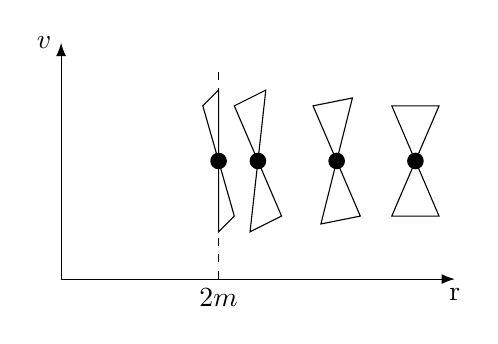
\begin{tikzpicture}
        \draw[-Latex] (-1,0) -- (4,0) node[anchor=north] {r};
        \draw[-Latex] (-1,0) -- (-1,3) node[anchor=east] {$v$};
        \fill (3.5,1.5) circle (3pt);
        \draw (3.2,0.8) -- (3.8,0.8) -- (3.2,2.2) -- (3.8,2.2) -- cycle;
        \fill (2.5,1.5) circle (3pt);
        \draw (2.3,0.7) -- (2.8,0.8) -- (2.2,2.2) -- (2.7,2.3) -- cycle;
        \fill (1.5,1.5) circle (3pt);
        \draw (1.4,0.6) -- (1.8,0.8) -- (1.2,2.2) -- (1.6,2.4) -- cycle;
        \draw[dashed] (1,0) node[anchor=north] {$2m$} -- (1,2.7);
        \fill (1,1.5) circle (3pt);
        \draw (1,0.6) -- (1.2,0.8) -- (0.8,2.2) -- (1,2.4) -- cycle;
    \end{tikzpicture}
\end{figure}
At large $r$, it always travels at 45 degrees.
The cones of influence are tipping over as the outward ray moves less and less, until we reach $r=2m$ and the outward propagating ray becomes purely time-like and cannot propagate outwards.
Once we're inside this radius, both light rays are then tipping over and both move towards the centre of the black hole as our term in Eq. (17.22) goes negative for both.
The zones of influence are aimed inwards to the Black Hole.

\chapter{}
\section{Initial Overview}
\begin{itemize}
    \item We had the \textbf{Principle of Equivalence} - all bodies feel the same gravity
    \item Mass $\implies$ curved space $\implies$ curved paths \emph{Yoda meme here}
    \item In Special Relativity, we had
        \begin{align}
            \begin{split}
                c^2d\tau^2 &= c^2dt^2 - dx^2 - dy^2 - dz^2 \\
                           &= \eta_{\alpha\beta}dx^\alpha dx^\beta,
            \end{split}
        \end{align}
        where we can express this using the Minkowski metric $\eta_{\alpha\beta}$.
    \item Einstein realised we can express this in a more general metric in General Relativity:
        \begin{align}
            c^2d\tau^2 &= g_{\alpha\beta}dx^\alpha dx^\beta,\quad g_{\alpha_\beta} = (\ve_{\alpha}\cdot\ve_{\beta}).
        \end{align}
    \item $\frac{\p\lambda^\beta}{\p x^\alpha} \implies \tensor{\lambda}{^\beta_{j\alpha}}$.
\end{itemize}

\section{Tensor Maths Toolkit}
We now need to figure out ways to represent everything in tensors.
This follows from defining contra- variant and covariant tensors respectively:
\begin{align}
    A^{\bar{b}} &= \frac{\p x^{\bar{b}}}{\p x^a}A^a, & A_{\bar{b}} &= \frac{\p x^a}{\p x^{\bar{b}}}A_a.
\end{align}
We can convert between these two forms using
\begin{align}
    \lambda_b &= g_{ab}\lambda^a,
\end{align}
where we need to remember we are using the Einstein Summation Convention over repeated indices.

\section{Geodesic paths and curved space}
When you move a tensor around in curved space, you get changes due to how the coordinate space changes.
To accommodate for this, we introduce the Total Derivative:
\begin{align}
    \frac{D\lambda^a}{ds} &= \frac{d\lambda^a}{ds} + \tensor{\Gamma}{^a_{bc}}\lambda^b\frac{dx^c}{ds} = \tensor{\lambda}{^a_{;c}}\frac{dx^c}{ds}, \\
    \tensor{\lambda}{^a_{;c}} &= \frac{\p\lambda^a}{\p x^c} + \tensor{\Gamma}{^a_{bc}}\lambda^b, \\
    \tensor{\Gamma}{^f_{bc}} &= \frac12 g^{bf}\left(\p_a g_{bc} - \p_b g_{ca} + \p_c g_{ab}\right).
\end{align}
We then introduce the concept of \emph{parallel transport}, which led us to geodesic paths:
\begin{align}
    \ddot{x}^a + \tensor{\Gamma}{^a_{bc}}\dot{x}^b\dot{x}^c = 0.
\end{align}
For working in equations of motion, we turn to the Euler-Lagrange equations.
So we express our Lagrangian and then write the E-L equation:
\begin{align}
    \La &= \frac12 g_{\alpha\beta}\dot{x}^\alpha\dot{x}^\beta, & \frac{d}{d\tau}\left(\frac{\p\La}{\p\dot{x}^a}\right) - \frac{\p\La}{\p x^\alpha} &= 0.
\end{align}
The definition of geodesic paths and Euler-Lagrange equation are equivalent, although generally we will find the E-L equation easier to work with.
This is all well and good, but then we realised that the Riemann curvature tensor $\tensor{R}{^a_{dbc}}$ was like the `second derivative' and can tell us a lot about space.
But we can't equate this with our other tensors yet.

\section{Einstein's Equations}
We want to describe how mass and the shape of space are related.
This is derived in the \textbf{Stress-Energy Tensor}:
\begin{align}
    T^{\mu\nu} &= \left(\rho_0+\frac{p}{c^2}\right)u^\mu u^\nu - Pg^{\mu\nu},
\end{align}
so the `00' element describes energy, and the other elements describe momentum.
In the last term above, we subtract by pressure to get the right form.
All of physics then can be written as
\begin{align}
    \tensor{T}{^{\mu\nu}_{;\mu}} &= 0.
\end{align}
To help equate different quantities, we introduce the Ricci tensor, which is a \emph{compressed} form of the Riemann tensor:
\begin{align}
    R_{\mu\nu} &= \tensor{R}{^\alpha_{\mu\nu\alpha}}.
\end{align}
We can then compress the Ricci tensor by performing its trace, yielding the \textbf{Curvature Scalar}:
\begin{align}
    \mathcal{R} &= \tensor{R}{^\alpha_\alpha}.
\end{align}
Einstein then used all this to define his `guess' as a way of writing down a relation between the curvature of space and the stress-energy:
\begin{align}
    \left(R^{\mu\nu}-\frac12 g^{\mu\nu}\mathcal{R}\right) &= \kappa T^{\mu\nu}.
\end{align}
Turns out this wasn't quite right - there is also a small \emph{cosmological constant} that needs to be added, which is famous for being Einstein's big blunder.
The metric is then useful to be redefined once we have reached this point, so we now introduce the Schwarzchild Metric, defining $m=\frac{GM}{c^2}$:
\begin{align}
    c^2d\tau^2 &= c^2\left(1-\frac{2m}{r}\right)\,dt^2 - \left(1-\frac{2m}{r}\right)^{-1}\,dr^2 - r^2d\theta^2 - r^2\sin^2\theta\,d\phi^2.
\end{align}
The rest of the lecture series was pretty much focused on how we solve this metric in different regimes.
\begin{itemize}
    \item Particles in weak gravity - here, we seemed to recover essentially Newtonian physics, with slight corrections. This resolved the perihelion of Mercury and was the first big success of GR.
    \item Photons in weak gravity - leading us to gravitational lensing and photons' movement.
    \item Orbits in strong gravity - the metric terms are no longer small as in weak gravity, more complex to solve.
    \item Radial paths in strong gravity.
    \item Alternative ways of writing the metric - looking at causality and where the metric should fail and how we fix that (i.e. inside $r=2m$).
\end{itemize}







\end{document}
